\documentclass{memoir}\usepackage[]{graphicx}\usepackage[]{color}
%% maxwidth is the original width if it is less than linewidth
%% otherwise use linewidth (to make sure the graphics do not exceed the margin)
\makeatletter
\def\maxwidth{ %
  \ifdim\Gin@nat@width>\linewidth
    \linewidth
  \else
    \Gin@nat@width
  \fi
}
\makeatother

\definecolor{fgcolor}{rgb}{0.345, 0.345, 0.345}
\newcommand{\hlnum}[1]{\textcolor[rgb]{0.686,0.059,0.569}{#1}}%
\newcommand{\hlstr}[1]{\textcolor[rgb]{0.192,0.494,0.8}{#1}}%
\newcommand{\hlcom}[1]{\textcolor[rgb]{0.678,0.584,0.686}{\textit{#1}}}%
\newcommand{\hlopt}[1]{\textcolor[rgb]{0,0,0}{#1}}%
\newcommand{\hlstd}[1]{\textcolor[rgb]{0.345,0.345,0.345}{#1}}%
\newcommand{\hlkwa}[1]{\textcolor[rgb]{0.161,0.373,0.58}{\textbf{#1}}}%
\newcommand{\hlkwb}[1]{\textcolor[rgb]{0.69,0.353,0.396}{#1}}%
\newcommand{\hlkwc}[1]{\textcolor[rgb]{0.333,0.667,0.333}{#1}}%
\newcommand{\hlkwd}[1]{\textcolor[rgb]{0.737,0.353,0.396}{\textbf{#1}}}%

\usepackage{framed}
\makeatletter
\newenvironment{kframe}{%
 \def\at@end@of@kframe{}%
 \ifinner\ifhmode%
  \def\at@end@of@kframe{\end{minipage}}%
  \begin{minipage}{\columnwidth}%
 \fi\fi%
 \def\FrameCommand##1{\hskip\@totalleftmargin \hskip-\fboxsep
 \colorbox{shadecolor}{##1}\hskip-\fboxsep
     % There is no \\@totalrightmargin, so:
     \hskip-\linewidth \hskip-\@totalleftmargin \hskip\columnwidth}%
 \MakeFramed {\advance\hsize-\width
   \@totalleftmargin\z@ \linewidth\hsize
   \@setminipage}}%
 {\par\unskip\endMakeFramed%
 \at@end@of@kframe}
\makeatother

\definecolor{shadecolor}{rgb}{.97, .97, .97}
\definecolor{messagecolor}{rgb}{0, 0, 0}
\definecolor{warningcolor}{rgb}{1, 0, 1}
\definecolor{errorcolor}{rgb}{1, 0, 0}
\newenvironment{knitrout}{}{} % an empty environment to be redefined in TeX

\usepackage{alltt}

\usepackage{hyperref}
\usepackage[all]{hypcap} 
\usepackage{enumitem, hyperref}
\usepackage{memhfixc}
\usepackage{bbding}
\usepackage{rotating}
\usepackage{changepage}
\usepackage{graphicx}
\usepackage{booktabs}
\usepackage{xspace}
\usepackage{listings}
\usepackage{float}
\usepackage{color}
\usepackage{titlesec}
\usepackage{xcolor}
\usepackage[T1]{fontenc}
\usepackage[utf8]{inputenc}


\usepackage[backend=bibtex]{biblatex}


\bibliography{references}

%\DeclareNameAlias{default}{last-first}
\DefineBibliographyStrings{english}{%
  references = {Works Cited},% replace "references" with "bibliography"  for `book`/`report`
}


\lstset{ %
  basicstyle=\ttfamily\footnotesize,       % the size of the fonts that are used for the code
  showspaces=false,               % show spaces adding particular underscores
  showstringspaces=false,         % underline spaces within strings
  showtabs=false,                 % show tabs within strings adding particular underscores
  tabsize=2,                      % sets default tabsize to 2 spaces
  captionpos=b,                   % sets the caption-position to bottom
  breaklines=true,                % sets automatic line breaking
  breakatwhitespace=false,        % sets if automatic breaks should only happen at whitespace
}

\lstnewenvironment{codelisting}[1][]%
  {\noindent\minipage{\linewidth}\medskip 
   \lstset{basicstyle=\ttfamily\footnotesize,#1}}
  {\endminipage}

%for list refs
\makeatletter
\def\namedlabel#1#2{\begingroup
    #2%
    \def\@currentlabel{#2}%
    \phantomsection\label{#1}\endgroup
}
\makeatother

%David's code
\let\proglang=\textsf
\newcommand{\pkg}[1]{{\fontseries{b}\selectfont #1}}
\let\code=\texttt 

\newcommand{\latex}{\LaTeX\xspace}

\setlength\heavyrulewidth{1.5pt}
	
\renewcommand*\cftappendixname{\appendixname}



\makeatletter
\newlength\drop
\newcommand*{\titleGM}{%
\thispagestyle{empty}
\begingroup% Gentle Madness
\drop = 0.1\textheight
\vspace*{\baselineskip}
\vfill
\hbox{%
  \hspace*{0.2\textwidth}%
  \rule{1pt}{\dimexpr\textheight-28pt\relax}%
  \hspace*{0.05\textwidth}% 
  \parbox[b]{0.75\textwidth}{%
    \vbox{%
      \vspace{\drop}
      {\Huge\bfseries\raggedright\@title\par}\vskip2.37\baselineskip
      {\Large\bfseries\@author\par}
      \vspace{0.5\textheight}
    }% end of vbox
  }% end of parbox
}% end of hbox
\vfill
\null
\endgroup}
\makeatother





\begin{filecontents*}{references.bib}
\begin{knitrout}
\definecolor{shadecolor}{rgb}{0.969, 0.969, 0.969}\color{fgcolor}\begin{kframe}
\begin{alltt}
\hlstd{bib} \hlkwb{=} \hlkwd{read.bib}\hlstd{(}\hlkwc{file} \hlstd{=} \hlstr{"references.bib"}\hlstd{)}
\end{alltt}


{\ttfamily\noindent\bfseries\color{errorcolor}{\#\# Error: could not find function "{}read.bib"{}}}\end{kframe}
\end{knitrout}
\end{filecontents*}

\title{Refactoring the xtable package}
\author{Daniel Geals}


\usepackage{chngcntr}
\counterwithout{footnote}{chapter}
\IfFileExists{upquote.sty}{\usepackage{upquote}}{}
\begin{document}








\frontmatter
\pagestyle{empty}
\aliaspagestyle{chapter}{empty}
%\titleGM

\calccentering{\unitlength}                         % Calculate center length and stores in unitlength
\begin{adjustwidth*}{\unitlength}{-\unitlength}     % Adjust center
    \begin{adjustwidth}{-1cm}{-1cm}
\begin{center}
\vspace{1cm}

%%% Type the thesis title below%%%%%%%%%%%%%%%%
{\Huge         Refactoring the xtable package}

\vspace{35mm} 


\includegraphics[width=2cm]{logo}

 \vspace{45mm}

%%%%%Type Your Name Below%%%%%%%%%%%%
{\Large       Daniel Geals}

  \vspace{1ex}

Department of Statistics

The University of Auckland

  \vspace{5ex}

 %%%%%Typing Your Supervisors Name Below%%%%%%%%%%%%
Supervisors: David Scott and Paul Murrell            

  \vspace{30mm}

A dissertation submitted in partial fulfilment of the requirements for the degree of BSc(Hons)  in Statistics, The University of Auckland, 2014.
\end{center}
   \end{adjustwidth}
\end{adjustwidth*}






\chapter*{Acknowledgements}
I would like to thank my supervisors David Scott and Paul Murrell for their frequent provision of direction and constructive assessment for the duration of this project. Their guidance was a highly significant factor in my enjoyment and completion of the project.

\newpage\leavevmode\thispagestyle{empty}\newpage

\chapter*{Abstract}
This project is about refactoring the \pkg{R} extension package, \pkg{xtable}. The first section will introduce \pkg{xtable} and present a case as to why such functionality, as the package provides, is useful. The next section is a survey of the R packages capable of producing similar table output. This will place \pkg{xtable} within the context of the R ecosystem by showing capabilities of other similarly tasked packages. It will also provide an overview of the features to which \pkg{xtable} has primarily been developed for. Following on is a section to illustrate current issues with \pkg{xtable}'s implementation and why it is important to refactor. This section also presents an overview of proper programming practice in relation to refactoring a program. Finally, the steps taken to modify the package will be presented and assessed.


\newpage\leavevmode\thispagestyle{empty}\newpage

\tableofcontents*

\mainmatter
\pagestyle{ruled}

\chapter{Introduction}


\section{Introduction to the xtable package}


The \pkg{xtable}\cite{xtable} package, authored by David B. Dahl,  is an R\cite{R} extension package that outputs formatted code for producing tables in \latex and HTML from a variety of R objects and classes. The package is primarily focused towards producing typeset \latex  tables for use in technical documents such as journal articles, academic documents and books. The HTML option has fewer arguments but is nonetheless useful for producing tables for usage in web, word processor and markdown documents. These capabilities make \pkg{xtable} especially useful for reproducible research purposes. Christopher Gandrud's \textit{Reproducible Research with R and RStudio}\cite{gan13} highlights that tables are useful tools for presentation of key statistics such as parameter estimates and descriptive statistics. Moreover, that the manual production of such tables is a slow and error prone process. These issues, of manual table production, are mitigated by table exporting packages such as \pkg{xtable}. Gandrud also provides examples of \pkg{xtable's} and other table packages' usage within reproducible documents\cite{gan13}. \pkg{xtable} is also mentioned on the CRAN (Comprehensive R Archive Network)\footnote{http://cran.r-project.org/} Task View for reproducible research.\footnote{http://cran.r-project.org/web/views/ReproducibleResearch.html}\\

The usefulness of the package is further depicted by the number of other R packages that rely on \pkg{xtable} in some capacity. On the CRAN web page for \pkg{xtable}\footnote{http://cran.r-project.org/web/packages/xtable/index.html}, there are over 30 packages that depend on \pkg{xtable} and at least 70 that either import or suggest \pkg{xtable}. The number of packages that have some reliance to \pkg{xtable} indicates that the package is important in the realm of formatted table production in R. This degree of reliance indicates it is important to have \pkg{xtable} implemented in a logical and easily maintainable format so that changes and bug fixes can be made easily and securely.\\ 

This package offers a balance between customisation and ease of use in that a basic table can be produced with a single command and argument, whilst a more customised table can be created by utilising the numerous additional arguments \pkg{xtable} has. With \pkg{xtable} we can produce quite complex tables that would require substantial \latex or HTML coding by relatively simple commands. In this way, the package is useful in the time it saves for producing these structured tables and in the potential errors that are avoided by outputting the table with correctly formatted alignment, columns, digits and so on, that arise in transcribing content to \latex or HTML table formats. 

\subsection{Examples of xtable usage}

This section will briefly demonstrate \pkg{xtable}'s main functionalities.

\vspace{1mm}


\begin{codelisting}[caption={logistic regression table input},language=R]
library(xtable)
fit = glm(Kyphosis ~ Age + I(Age^2) + Number + Start,
          family = binomial, data = kyphosis)
xtable(summary(fit), caption = 
	"Logistic regression with kyphosis data set",
  label = "tbl:logistic")
\end{codelisting}

% latex table generated in R 3.1.1 by xtable 1.7-3 package
% Thu Nov 20 18:39:28 2014
\begin{table}[ht]
\centering
\begin{tabular}{rrrrr}
  \hline
 & Estimate & Std. Error & z value & Pr($>$$|$z$|$) \\ 
  \hline
(Intercept) & -4.3836 & 2.0549 & -2.13 & 0.0329 \\ 
  Age & 0.0816 & 0.0345 & 2.36 & 0.0181 \\ 
  I(Age\verb|^|2) & -0.0004 & 0.0002 & -2.08 & 0.0374 \\ 
  Number & 0.4269 & 0.2365 & 1.80 & 0.0711 \\ 
  Start & -0.2038 & 0.0707 & -2.88 & 0.0039 \\ 
   \hline
\end{tabular}
\caption{Logistic regression with kyphosis data set} 
\label{tbl:logistic}
\end{table}



\begin{codelisting}[caption={random data table input},language=R]
library(xtable)
words = rep(c("low", "medium", "high") ,3)
x = data.frame(var1 = rnorm(n = 9, mean = 10, sd = 2),
  	var2 = rnorm(n = 9, mean = 5, sd = 15),
		var3 = runif(n = 9, min = -4, max = 4),
		var4 = rnorm(n = 9, mean = 0, sd = 100),
		factor = factor(sample(words)))
tbl = xtable(x, digits = 2, 
  caption = "data frame of random data with booktabs option",
  label = "tbl:random")
align(tbl) = c("|lr|r|r|r|l|")
print(tbl, booktabs = TRUE)
\end{codelisting}

% latex table generated in R 3.1.1 by xtable 1.7-3 package
% Thu Nov 20 18:39:28 2014
\begin{table}[ht]
\centering
\begin{tabular}{|lr|r|r|r|l|}
  \toprule
 & var1 & var2 & var3 & var4 & factor \\ 
  \midrule
1 & 6.75 & -1.30 & -3.19 & 60.52 & low \\ 
  2 & 9.52 & -2.29 & -2.24 & -139.13 & medium \\ 
  3 & 10.49 & 26.74 & -3.74 & -33.22 & high \\ 
  4 & 5.53 & -9.17 & 2.27 & 61.12 & low \\ 
  5 & 10.22 & 15.31 & -0.72 & -11.83 & high \\ 
  6 & 9.29 & 5.24 & -0.30 & -8.10 & low \\ 
  7 & 6.90 & 22.49 & 0.89 & 49.00 & medium \\ 
  8 & 10.96 & 13.03 & 0.77 & -161.62 & high \\ 
  9 & 11.29 & -0.20 & 2.43 & -2.55 & medium \\ 
   \bottomrule
\end{tabular}
\caption{data frame of random data with booktabs option} 
\label{tbl:random}
\end{table}



\newpage

Below is the \latex output for table \ref{tbl:random} before being processed.

\vspace{3mm}
\begin{codelisting}[caption={latex table via xtable},language=R]
% latex table generated in R 3.1.1 by xtable 1.7-3 package
% Sat Oct 11 09:54:29 2014
\begin{table}[ht]
\centering
\begin{tabular}{|lr|r|r|r|l|}
  \toprule
 & var1 & var2 & var3 & var4 & factor \\
  \midrule
 1 & 9.93 & 7.12 & -3.84 & 71.28 & low \\
 2 & 11.26 & 4.31 & 2.17 & 140.38 & high \\
 3 & 11.71 & 5.37 & 3.17 & 56.01 & medium \\
 4 & 9.95 & 34.41 & 0.43 & 16.25 & low \\
 5 & 9.04 & 18.55 & 2.18 & 16.47 & high \\
 6 & 10.27 & -17.29 & -2.37 & 40.05 & medium \\
 7 & 10.54 & -1.86 & 3.20 & 17.62 & low \\
 8 & 9.84 & -7.17 & 1.87 & 45.73 & high \\
 9 & 9.19 & 1.55 & -2.24 & -120.06 & medium \\
 10 & 11.53 & 4.09 & -3.84 & 86.78 & low \\
 11 & 8.37 & -46.66 & 3.64 & -11.83 & high \\
 12 & 12.12 & -23.79 & 1.76 & 274.48 & medium \\
  \bottomrule
\end{tabular}
\caption{data frame of simulated data with booktabs option}
\end{table}
\end{codelisting}

\vspace{3mm}

This output and resulting table demonstrate the usefulness of packages for producing \latex and HTML content. With \pkg{xtable}, content can be produced more easily, more quickly and with less error in comparison to coding 'by hand'. 


\newpage

\section{Survey of \latex and HTML table exporting packages}

Hosted on CRAN are many R packages possessing functionality related to coercing R objects into \latex or HTML tables. It is worth considering what exactly these functionalities are, comparing functionality across these related packages and seeing how \pkg{xtable} fits into this group of packages. By surveying the packages available and making comparisons, evidence of \pkg{xtable}'s utility is shown. The comparisons are made by tabling the results of the survey.

\vspace{4mm}

\textbf{Survey method:}
The data in these tables were largely collected by examining package documentation. For the "objects" table the methods of functions were occasionally examined in R. This clarification was undertaken if the R documentation was not comprehensive or clear. The "features" tables data were found also by examination of documentation; through looking at the arguments of functions relating to \latex and HTML output.

\vspace{10 pt}

\subsection{Packages versus input objects}

Table \ref{fig:objects} shows packages against the objects that can be used to produce formatted output in \latex or HTML. This is not an exhaustive list of objects that these packages accept, some packages accept objects other than those shown. For instance, \pkg{stargazer}\cite{stargazer} and \pkg{texreg}\cite{texreg} can both produce output using an extensive array of model objects. Moreover, the packages listed here are not exhaustive. There are a number of packages that have HTML and \latex table production capabilities but have not been included if they are too specific or too limited for the purposes of this survey. Packages that are too specific are those that are specialised for tasks other than table production and have table publication output for a unique object created by the package. For example:

\begin{itemize}
\item \pkg{FactoClass}\cite{FactoClass}: this package is for combination of factorial methods and cluster analysis. It has a couple of \latex functions: \code{dudi.tex} and \code{FactoClass.tex} that are used to output results or tables specific to factorial methods and cluster analysis. 
\item \pkg{bpca}\cite{bpca}: this package creates biplots of multivariate data based on PCA. It has functions called \code{latex.bpca} that returns a biplot, and a function called \code{summary.latex.bpca} that returns a summary in LaTeX.
\item \pkg{BoolNet}\cite{BoolNet}: this package's functionality is Boolean networks. It has latex functions: \code{attractorsToLaTeX} and \code{sequenceToLatex}. These both produce tables using specific objects and analysis from the package.
\end{itemize}
\vspace{10 pt} 
Packages that are too limited typically have some small \latex or HTML function with few inputs and outputs. Examples of such packages are:
\begin{itemize}
\item  \pkg{miscFuncs}\cite{miscFuncs}: this miscellaneous function package has a \code{latextable} function that only creates tables from matrices and has the basic but important arguments such as digits, colnames, rownames, caption, NA replacement. It does have a scientific notation for very small numerical figures, which doesn't seem to be a common feature amongst other packages.
\item \pkg{sfsmisc}\cite{sfsmisc}: this is another miscellaneous function package with a considerable number of functions but with \latex table functions only for matrices and with limited features
\end{itemize}


\begin{table}[ht]
 \vspace{50pt} \scalebox{0.8}{
\begin{tabular}{*{16}{r}}
Packages.v.Inputs & \begin{rotate}{90}  data.frame \end{rotate} & \begin{rotate}{90}  matrix \end{rotate} & \begin{rotate}{90}  lm \end{rotate} & \begin{rotate}{90}  coxph \end{rotate} & \begin{rotate}{90}  summary \end{rotate} & \begin{rotate}{90}  glm \end{rotate} & \begin{rotate}{90}  lme \end{rotate} & \begin{rotate}{90}  aov \end{rotate} & \begin{rotate}{90}  ftable \end{rotate} & \begin{rotate}{90}  table \end{rotate} & \begin{rotate}{90}  mtable \end{rotate} & \begin{rotate}{90}  xtab \end{rotate} & \begin{rotate}{90}  ts \end{rotate} & \begin{rotate}{90}  zoo \end{rotate} & \begin{rotate}{90}  prcomp \end{rotate}\\
\hline
xtable & \CheckmarkBold & \CheckmarkBold & \CheckmarkBold & \CheckmarkBold & \CheckmarkBold & \CheckmarkBold &  & \CheckmarkBold &  & \CheckmarkBold &  & \CheckmarkBold & \CheckmarkBold & \CheckmarkBold & \CheckmarkBold\\
\hline
R2HTML & \CheckmarkBold & \CheckmarkBold & \CheckmarkBold & \CheckmarkBold & \CheckmarkBold &  &  & \CheckmarkBold & \CheckmarkBold & \CheckmarkBold &  & \CheckmarkBold & \CheckmarkBold &  & \CheckmarkBold\\
\hline
stargazer & \CheckmarkBold &  & \CheckmarkBold & \CheckmarkBold & \CheckmarkBold & \CheckmarkBold & \CheckmarkBold & \CheckmarkBold &  &  &  &  &  &  & \\
\hline
rms &  &  & \CheckmarkBold & \CheckmarkBold & \CheckmarkBold &  &  & \CheckmarkBold &  &  &  &  &  &  & \\
\hline
apsrtable &  &  & \CheckmarkBold & \CheckmarkBold & \CheckmarkBold & \CheckmarkBold &  &  &  &  &  &  &  &  & \\
\hline
texreg &  &  & \CheckmarkBold & \CheckmarkBold &  & \CheckmarkBold & \CheckmarkBold &  &  &  &  &  &  &  & \\
\hline
memisc &  & \CheckmarkBold & \CheckmarkBold &  &  &  &  &  & \CheckmarkBold &  & \CheckmarkBold &  &  &  & \\
\hline
Hmisc & \CheckmarkBold & \CheckmarkBold &  &  &  &  &  &  & \CheckmarkBold &  &  &  &  &  & \\
\hline
taRifx & \CheckmarkBold &  & \CheckmarkBold &  &  &  & \CheckmarkBold &  &  &  &  &  &  &  & \\
\hline
fdth & \CheckmarkBold & \CheckmarkBold &  &  &  &  &  &  &  &  &  &  &  &  & \\
\hline
hwriter & \CheckmarkBold & \CheckmarkBold &  &  &  &  &  &  &  &  &  &  &  &  & \\
\hline
rockchalk &  &  & \CheckmarkBold &  &  & \CheckmarkBold &  &  &  &  &  &  &  &  & \\
\hline
quantreg &  & \CheckmarkBold &  &  & \CheckmarkBold &  &  &  &  &  &  &  &  &  & \\
\hline
reporttools & \CheckmarkBold &  &  & \CheckmarkBold &  &  &  &  &  &  &  &  &  &  & \\
\hline
hwriterPlus & \CheckmarkBold & \CheckmarkBold &  &  &  &  &  &  &  &  &  &  &  &  & \\
\hline
suRtex & \CheckmarkBold & \CheckmarkBold &  &  &  &  &  &  &  &  &  &  &  &  & \\
\hline
r2lh & \CheckmarkBold &  &  &  &  &  &  &  &  &  &  &  &  &  & \\
\hline
tables & \CheckmarkBold &  &  &  &  &  &  &  &  &  &  &  &  &  & \\
\hline
etable & \CheckmarkBold &  &  &  &  &  &  &  &  &  &  &  &  &  & \\
\hline
 \end{tabular}
}\caption{Packages versus Input Objects}
\label{fig:objects}
\end{table}




Some features of table \ref{fig:objects} are:
\begin{itemize}
\item The majority of packages can produce output using data frame objects
\item There are packages that mainly accept model type input, from objects such as lm, summary and coxph. Examples of this type of package are \pkg{apsrtable}\cite{apsrtable}, \pkg{rms}\cite{rms} and \pkg{stargazer}. In fact packages such as \pkg{texreg}\cite{texreg} and \pkg{stargazer} are specialised towards model output and can accept a wide variety of model types as input. This model specialisation is quite distinct from the more general aims of \pkg{xtable}.
\item There are packages that are more limited in the number objects accepted and mainly focus on data frame. These generally are packages focused on descriptive statistics and/or are packages that are utility types. Examples of this type are \pkg{etable}\cite{etable} and \pkg{Hmisc}\cite{Hmisc}.
\item Two packages that utilise the widest range of objects are \pkg{xtable} and \pkg{R2HTML}\cite{R2HTML}. These packages seem to have a wider functionality than other packages with focus on both descriptive and modelling table production.
\end{itemize}


\subsection{Packages versus features:}

\vspace{10 pt}

Tables \ref{fig:latex} and \ref{fig:html} show the features of the packages broken down by \latex and HTML. The \latex table, \ref{fig:latex} only includes the packages from the objects table, table \ref{fig:objects}, that produce \latex output. Likewise, the HTML table, \ref{fig:html} only includes output from the packages from the objects table that produce HTML output. The features here are listed completely separately from the input object capabilities, so a package could have a limited number of features but still produce output from a wide variety of objects. That is to say some packages have the advantage of accepting many object classes, whilst others have the advantage of more more output customisation.\\


\textbf{\latex package features}


\begin{table}[ht]
 \vspace{50pt} \hspace*{-1cm}
\scalebox{0.8}{
\begin{tabular}{*{19}{r}}
LaTeXFeatures & \begin{rotate}{90}  dec.pl \end{rotate} & \begin{rotate}{90}  colnames \end{rotate} & \begin{rotate}{90}  rownames \end{rotate} & \begin{rotate}{90}  Caption \end{rotate} & \begin{rotate}{90}  label \end{rotate} & \begin{rotate}{90}  alignment \end{rotate} & \begin{rotate}{90}  headings \end{rotate} & \begin{rotate}{90}  size \end{rotate} & \begin{rotate}{90}  float \end{rotate} & \begin{rotate}{90}  longtable \end{rotate} & \begin{rotate}{90}  Dcolumn \end{rotate} & \begin{rotate}{90}  booktabs \end{rotate} & \begin{rotate}{90}  Lines \end{rotate} & \begin{rotate}{90}  center \end{rotate} & \begin{rotate}{90}  width \end{rotate} & \begin{rotate}{90}  spanning \end{rotate} & \begin{rotate}{90}  Initial.Zero \end{rotate} & \begin{rotate}{90}  bold \end{rotate}\\
\hline
xtable & \CheckmarkBold & \CheckmarkBold & \CheckmarkBold & \CheckmarkBold & \CheckmarkBold & \CheckmarkBold &  & \CheckmarkBold & \CheckmarkBold & \CheckmarkBold &  & \CheckmarkBold & \CheckmarkBold & \CheckmarkBold & \CheckmarkBold &  &  & \\
\hline
Hmisc & \CheckmarkBold & \CheckmarkBold & \CheckmarkBold & \CheckmarkBold & \CheckmarkBold & \CheckmarkBold & \CheckmarkBold & \CheckmarkBold &  & \CheckmarkBold & \CheckmarkBold & \CheckmarkBold & \CheckmarkBold & \CheckmarkBold & \CheckmarkBold &  &  & \\
\hline
texreg & \CheckmarkBold & \CheckmarkBold & \CheckmarkBold & \CheckmarkBold & \CheckmarkBold &  &  & \CheckmarkBold & \CheckmarkBold &  & \CheckmarkBold & \CheckmarkBold & \CheckmarkBold & \CheckmarkBold &  &  & \CheckmarkBold & \CheckmarkBold\\
\hline
reporttools &  & \CheckmarkBold & \CheckmarkBold & \CheckmarkBold & \CheckmarkBold &  &  & \CheckmarkBold &  & \CheckmarkBold &  &  &  &  &  &  &  & \\
\hline
tables & \CheckmarkBold & \CheckmarkBold & \CheckmarkBold &  &  & \CheckmarkBold & \CheckmarkBold &  &  & \CheckmarkBold &  & \CheckmarkBold &  &  &  & \CheckmarkBold &  & \\
\hline
quantreg & \CheckmarkBold & \CheckmarkBold & \CheckmarkBold & \CheckmarkBold & \CheckmarkBold &  &  &  &  & \CheckmarkBold & \CheckmarkBold &  &  &  &  &  &  & \\
\hline
apsrtable & \CheckmarkBold & \CheckmarkBold & \CheckmarkBold & \CheckmarkBold & \CheckmarkBold & \CheckmarkBold &  &  & \CheckmarkBold &  & \CheckmarkBold &  &  &  &  & \CheckmarkBold &  & \\
\hline
stargazer & \CheckmarkBold & \CheckmarkBold & \CheckmarkBold & \CheckmarkBold & \CheckmarkBold & \CheckmarkBold & \CheckmarkBold & \CheckmarkBold & \CheckmarkBold &  &  &  & \CheckmarkBold &  &  &  & \CheckmarkBold & \\
\hline
taRifx & \CheckmarkBold &  &  & \CheckmarkBold & \CheckmarkBold & \CheckmarkBold &  &  &  &  &  &  &  &  &  &  &  & \\
\hline
rms & \CheckmarkBold & \CheckmarkBold &  & \CheckmarkBold &  &  &  & \CheckmarkBold &  &  &  &  &  &  &  &  &  & \\
\hline
memisc & \CheckmarkBold &  &  &  &  &  & \CheckmarkBold &  &  &  & \CheckmarkBold & \CheckmarkBold &  &  &  &  &  & \\
\hline
fdth &  &  &  & \CheckmarkBold & \CheckmarkBold & \CheckmarkBold &  & \CheckmarkBold &  &  &  &  &  &  &  &  &  & \\
\hline
suRtex & \CheckmarkBold &  &  & \CheckmarkBold &  &  &  &  &  &  &  &  &  &  &  &  &  & \\
\hline
rockchalk & \CheckmarkBold & \CheckmarkBold & \CheckmarkBold &  & \CheckmarkBold &  & \CheckmarkBold &  & \CheckmarkBold &  &  &  &  &  &  &  &  & \\
\hline
etable &  & \CheckmarkBold & \CheckmarkBold &  &  &  &  &  &  &  &  &  &  &  &  &  &  & \\
\hline
r2lh &  &  &  & \CheckmarkBold &  &  &  &  &  &  &  &  &  &  &  &  &  & \\
\hline
 \end{tabular}
}
\hspace*{-1.5cm}
\caption{LaTeX Packages and Output Features}
\label{fig:latex}
\end{table}




Table \ref{fig:latex} shows a number of the most common features of the output produced from the \latex specific functions of each package of interest. Again, this is not an exhaustive list of the features that these packages are capable of producing. It is a sample of the most common features seen when looking through package documentation of the \latex specific functions. The most common features related to the decimal places (dec.pl or digits) of numerical content, customisation of row and columns (names, show or hide, rotation and so on),  caption and labels, alignment, headings and size. 

There are a number of packages with a large number of features allowing for considerable customisation of output. The packages with the most customisation of output are: \pkg{xtable}, \pkg{Hsmic} and \pkg{texreg}.\\


\textbf{HTML package features}

\begin{table}[ht]
 \vspace{50pt} \hspace*{-1cm}
\scalebox{0.75}{
\begin{tabular}{*{20}{r}}
HTMLFeatures & \begin{rotate}{90}  caption \end{rotate} & \begin{rotate}{90}  rownames \end{rotate} & \begin{rotate}{90}  colnames \end{rotate} & \begin{rotate}{90}  alignment \end{rotate} & \begin{rotate}{90}  tags \end{rotate} & \begin{rotate}{90}  css \end{rotate} & \begin{rotate}{90}  spacing \end{rotate} & \begin{rotate}{90}  dec.pl \end{rotate} & \begin{rotate}{90}  center \end{rotate} & \begin{rotate}{90}  nesting \end{rotate} & \begin{rotate}{90}  colours \end{rotate} & \begin{rotate}{90}  Border \end{rotate} & \begin{rotate}{90}  Width \end{rotate} & \begin{rotate}{90}  title \end{rotate} & \begin{rotate}{90}  size \end{rotate} & \begin{rotate}{90}  bold \end{rotate} & \begin{rotate}{90}  to.file \end{rotate} & \begin{rotate}{90}  Lines \end{rotate} & \begin{rotate}{90}  MathJax \end{rotate}\\
\hline
hwriterPlus &  & \CheckmarkBold & \CheckmarkBold & \CheckmarkBold & \CheckmarkBold & \CheckmarkBold & \CheckmarkBold &  & \CheckmarkBold & \CheckmarkBold & \CheckmarkBold & \CheckmarkBold & \CheckmarkBold & \CheckmarkBold & \CheckmarkBold &  &  &  & \CheckmarkBold\\
\hline
hwriter &  & \CheckmarkBold & \CheckmarkBold & \CheckmarkBold & \CheckmarkBold & \CheckmarkBold & \CheckmarkBold &  & \CheckmarkBold & \CheckmarkBold & \CheckmarkBold & \CheckmarkBold & \CheckmarkBold &  &  &  &  &  & \\
\hline
stargazer & \CheckmarkBold & \CheckmarkBold & \CheckmarkBold & \CheckmarkBold &  &  & \CheckmarkBold & \CheckmarkBold &  &  &  &  &  & \CheckmarkBold & \CheckmarkBold &  &  & \CheckmarkBold & \\
\hline
texreg & \CheckmarkBold &  &  &  & \CheckmarkBold & \CheckmarkBold &  & \CheckmarkBold & \CheckmarkBold &  &  &  &  &  &  & \CheckmarkBold &  &  & \\
\hline
tables &  &  &  & \CheckmarkBold & \CheckmarkBold & \CheckmarkBold & \CheckmarkBold &  &  &  &  &  &  &  &  &  &  &  & \\
\hline
R2HTML & \CheckmarkBold & \CheckmarkBold &  &  &  &  &  & \CheckmarkBold &  &  &  & \CheckmarkBold &  &  &  &  &  &  & \\
\hline
xtable & \CheckmarkBold & \CheckmarkBold & \CheckmarkBold &  &  &  &  &  &  &  &  &  &  &  &  &  &  &  & \\
\hline
r2lh & \CheckmarkBold &  &  &  &  &  &  &  &  &  &  &  &  &  &  &  &  &  & \\
\hline
rockchalk &  &  &  &  &  &  &  &  &  &  &  &  &  &  &  &  & \CheckmarkBold &  & \\
\hline
Hmisc &  &  &  &  &  &  &  &  &  &  &  &  &  &  &  &  &  &  & \\
\hline
 \end{tabular}
}
\hspace*{-1cm}
\caption{HTML Packages and Output Features}
\label{fig:html}
\end{table}



Table \ref{fig:html} shows features produced by the packages shown in \ref{fig:objects}, with HTML production capabilities. The most prolific packages in terms of output options are \pkg{hwriterPlus}\cite{hwriterPlus}, \pkg{hwriter}\cite{hwriter} and \pkg{stargazer}. The most common features are captions, row and column names, alignment, production of various HTML tags, CSS output, spacing or padding, and digits or decimal places. Note, \pkg{Hmisc} seems to have an extremely limited number of HTML features but does still produces HTML output, hence the empty row for \pkg{Hmisc}.

\newpage

\chapter{What is the problem}

\section{Issues with \pkg{xtable}}
\label{sec:issues}

The primary issue with \pkg{xtable} is the complex and unrefined implementation of one function, \code{print.xtable}. This function takes user inputs, including the object (data frame, lm summary, matrix, ...) to be coerced to a table, and prints the final \latex or HTML. The object, of the form: \code{xtable.object.class}, passed into \code{print.xtable} is created by a function from the file \code{xtable.R}. The function, \code{print.xtable}, was examined via debugging and by writing pseudo-code. 

\vspace{4mm}

There are several sources of complication for \code{print.xtable}

\begin{description}[style=multiline, labelwidth=0.5cm]
    \item[\namedlabel{itm:problem1}{1}] HTML and \latex functionality is bundled together so that the function will work for both formats.
    \item[\namedlabel{itm:problem2}{2}] It has been built up, quite significantly, over the years by adding requested features to this single function. You can look back to the \pkg{xtable} version 1.0-1 released in the year 2000 and see that \code{print.xtable} has roughly the same programmatic structure that exists currently.\footnote{See http://cran.r-project.org/src/contrib/Archive/xtable/ for previous \pkg{xtable} versions}
    \item[\namedlabel{itm:problem3}{3}] The code doesn't seem to have been cleaned up or refactored during its development. This relates closely to problem \ref{itm:problem2}, but it seems that generally a new piece of functionality is added part way through the function and has routines such as user input validation added into the code at the same location. This is evident in the comments of the code where there are commented out code chunks seemingly left for years and that we also have user input validation in places such as half-way through the function.
    \item[\namedlabel{itm:problem4}{4}] There are almost no functions created or referenced (\code{sanitize} is the only exception) within \code{print.xtable}. The lack of abstraction makes it hard to judge what the function is doing because you have to delve into the details.
    \item[\namedlabel{itm:problem5}{5}] There is a huge argument list(not to mention the function \code{xtable} has its own rather large argument list). The magnitude of the argument list, at 32 arguments, is borne out of the large amount of customisation that can be done within the various \latex table environments. The number of arguments makes it difficult for us to easily create functions without requiring a similarly large number of arguments.
    \item[\namedlabel{item:problem6}{6}] There is comprehensive test suite to validate the functionality of the function.
\end{description}


In order to get an idea of what the \code{print.xtable} function looks like, and roughly how it works we have a pseudo-code representation below. 

\begin{figure}[h!]
\begin{knitrout}
\definecolor{shadecolor}{rgb}{0.969, 0.969, 0.969}\color{fgcolor}

{\centering \includegraphics[width=\maxwidth]{figure/ok} 

}



\end{knitrout}
	\caption{psuedo-code of \code{print.xtable}}\label{fig:pseudo}
\end{figure}


 This summarises the steps undertaken when we call \code{print.xtable}. The line numbers give an indication of the level of detail hidden in this summary. So, this is a view of the function at quite a high level. The pseudo-code shows that the amount of activity and low level detail in this function is too high. This is not conducive to our understanding of the function which ultimately impacts maintenance and further extension of the package. This is especially an issue because \code{print.xtable} sits at the core of the \pkg{xtable} package.
 
 
\subsection{Problems of maintenance}

Issues with the \code{print.xtable} function cause us difficulties in maintenance and modification of the code. If there is an issue it will take longer for us to modify or fix bugs because locating the source of issues can take more time. Furthermore, without a test suite it is onerous to verify that our modifications are fully functional and bug free. It seems then, that over the course of development, less than ideal standards of programming practice have been adhered to. 
In addressing this issue, what exactly proper programming practice is, within our context and refactoring limitations, should be considered.

\section{Proper programming practice}\label{sec:practice}

Before embarking on the task of altering the package it would be ideal for us to consider what best practice is. By identifying proper programming practice and applying it to \pkg{xtable} we should be able to alleviate some of the issues as highlighted in section \ref{sec:issues}.

%possibly get page numbers for these references?

\begin{description}[style=multiline, labelwidth=2cm]
	\item[\namedlabel{itm:p1}{functions}] Functions should not be overly long and should do one or very few things. In Chapter 3 of Robert C. Martin's \textit{Clean Code} (2008), we see that functions that do a large number of operations and contain a lot of low level code are more difficult to understand.\cite{mar08}
	\item[\namedlabel{itm:p2}{abstraction}] Low level details should be hidden away within functions. This allows users to go through the code and understand it without having to unpack the details of the logic and operations. They can see an object is created at a specific point, via some function, and not need to have looked at the code that produced the object.
	\item[\namedlabel{itm:p3}{naming}] Following on from abstraction, the names of functions are important for allowing the code to be readable. In combination with a function's variables, the name should allow the reader to gain an understanding of what a function is doing. In \textit{Clean Code}, Martin (2008) dedicates all of the second chapter to discussing the importance of naming and various strategies to employ.\cite{mar08}
    \item[\namedlabel{itm:p3a}{modularity}] Related to the concept of abstraction is that of modularity. Whereby a program should be composed of distinct 'modules'.\cite{woo82} These 'modules' should have specifically grouped functionality to allow a reader to understand what is going on in a particular section of the program.
	\item[\namedlabel{itm:p4}{style}] Following a coding style. Be it in R or any other language, having a consistent style of coding applied will allow readers to understand the program more easily
	\item[\namedlabel{itm:p5}{comments}] Martin (2008) in chapter 4  explains that functions should not be cluttered with comments that are not helpful or currently useful.\cite{mar08} For instance, unused code that has been commented out will make the code bloated and potentially cause the reader to wonder if this code was implemented, abandoned or ready to be used.
	\item[\namedlabel{itm:p6}{validation}] User input should be thoroughly validated and understandable error messages should be returned.\cite{ibm} Whilst having a few of the obvious user input validations is useful, it seems that when we have so many combinations of arguments possible, which don't all work, it is necessary to have a thorough validating functionality to inform users of what they can use and why a particular use of the package wouldn't work.
	\item[\namedlabel{itm:p7}{testing}] Testing: in order to develop a package we know works it should be developed in tandem with testing procedures.\cite{testthat} We want to know that what we implement will work with the existing code base. This is especially true for a function with numerous arguments that can be used in various combinations because there are many more places the code may not work.
\end{description}


\section{Potential solutions}

Possible solutions for adapting \code{print.xtable} towards our requirements can essentially be restricted to two options. Rewriting the function of issue, or refactoring the current implementation. Both approaches would be attempted with goals of the resultant package being more comprehensible, maintainable and expandable in mind. These two approaches have their own positives and negatives.

\vspace{4mm}

\textbf{Rewriting} the package involves, at a minimum, a complete rewrite of the \code{print.xtable} function.\\

\noindent Advantages of rewriting:
\begin{itemize}
\item Being able to write the package and eliminate issues of the current implementation
\item Being unrestricted by the previous implementation of the package
\end{itemize}
Disadvantages of rewriting:
\begin{itemize}
\item potentially not understanding how features of table output are created; which could lead to an implementation that isn't suitable for producing certain table features.
\item difficulty of implementation. It is a lot of work to get the pre-existing arguments producing correct output whilst also achieving an achieving the initial goals of improvement. 
\item loss of backwards compatibility. This is important due to the number of people using the package; who will require previously compilable or runnable code to still be so.
\item to address the loss of backwards compatibility a new package would need to be released. This would mean a fractured user base and further issues surrounding supporting the previous iteration of \pkg{xtable} and also supporting the new \code{xtable2}.
\item In implementing a new package, the store of knowledge added to the existing package is partially or fully thrown away. This is wasteful due to the amount of work undertaken during the development of the package.
\end{itemize}

\textbf{Refactoring} the package involves reorganising the structure and details of the function, \code{print.xtable}, to be more understandable and maintainable.\\%rephrase this

\noindent Advantages of refactoring:
\begin{itemize}
\item We keep much of the work undertaken up to \pkg{xtable's} current iteration. We are not wasting resources doing reimplementation. Unless drastically changing the functionality of a package, in the case of there being a severe issue, we do not want to waste other peoples work.
\item By refactoring we will be able to provide and expose a greater understanding of how this function operates. This will be especially beneficial if a rewrite is eventually undertaken because it provides insight into the mechanisms generating certain features of a table.
\end{itemize}
Disadvantages of refactoring:
\begin{itemize}
\item We are limited in the extent of improvement that can be achieved because refactoring involves making use of the previous implementation.
\item We have to be extremely careful that our adjustments to the package have not broken some functionality. This is quite important in the case of \pkg{xtable}, which has so many arguments that will still need to work. This means that extra precautions must be taken to ensure backwards compatibility.
\end{itemize}

Given these advantages and disadvantages it seems logical that before any new package can be made, the current implementation should be refactored and analysed. In doing this it will be possible to gain insight into how the package works and what can be done to improve it. 

\chapter{Refactoring xtable}

%%not sure if this part is necessary at all
This section is about the details of refactoring \pkg{xtable}. The intention is to go through how the function \code{print.xtable} was refactored, along with the reasons and results of each successive refactoring step. To provide a brief overview: the overall process was to first implement a testing routine, then separate out detail of \code{print.xtable} into internal functions and finally split the remaining main \code{print.xtable} function into smaller parts.

\section{Testing methodology}

A preliminary task in the process of refactoring the \code{print.xtable} function was to set up a thorough and convenient testing procedure. Due to the high usage and employment of many of the additional arguments provided by \pkg{xtable} it is essential for any modifications to be tested. For development purposes, simply running the modified or refactored \pkg{xtable} with a few different argument types is insufficient; a particular combination of arguments could produce an error. If an error isn't caught it could be unknowingly incorporated into the refactored code. The test setup used to prevent this has two components: the first confirms output is correct, the second is to test that invalid user input is being rejected.\\ 


The first method, to test the package is working correctly, makes use of the \pkg{xtable} vignette\footnote{http://cran.r-project.org/web/packages/xtable/vignettes/xtableGallery.pdf} (a \latex gallery of \pkg{xtable} examples utilising a variety of arguments). The vignette or gallery contains many examples of \pkg{xtable} usage; by reprocessing this file we can see if the modifications have been successful or, to varying degrees, unsuccessful. The aim was to be able to compile the gallery with the refactored package and compare it to the gallery produced by the original package. This comparison is made by a diff utility, a utility that enables a line by line comparison of two files.

The files used to create the gallery are provided with the package source files. In this case the gallery file is in the \code{Sweave} file format, \code{.swn}.\footnote{the \pkg{xtable} gallery has recently been updated to \pkg{knitr}} Sweave allows for a single document with a mixture of R and \latex code to be compiled to a PDF file. The \code{Sweave} file is processed by the R function \code{Sweave}, combining the R and \latex components into a \code{.tex} file which is then used to create the gallery PDF. The \latex file, in \code{.tex} format, is the file, of the formats mentioned, to which the diff utility is applied. In this format we have the \latex from \pkg{xtable} and can see if the newly created gallery contains the correct \latex output. 

To setup the test; an 'original' \code{.tex} file is created with the unmodified \pkg{xtable}. To test if refactoring has been successful we run \code{Sweave} with the modified package and apply the diff utility to this modified gallery \code{.tex} file and the 'original' file. The utility will return nothing if the modified version is identical to the 'original', otherwise it will return locations of the different lines and we can attempt to find the source of error. To ensure the diff utility only returned output when there was a material change, the random variate examples were made non-random and the \pkg{xtable} timestamp option was turned off. This allowed for a fast check to confirm that modifications were not breaking \pkg{xtable}.\\


%testthat explanation seems fine
The second method was to create tests using the \pkg{testthat} package\cite{testthat}. Due to the customisable nature of \pkg{xtable} there are a large number of arguments. Many of these arguments cannot be used in conjunction with each other because of the non-compatible nature of certain \latex environments. It is therefore necessary to check that the user input validation sections are returning errors or warnings for invalid user input. Otherwise, the invalid input might cause incomprehensible errors when the function runs or when the resulting \latex or HTML is compiled. These tests were created to be put within the package and make running the tests convenient (they can be run via \code{test()} in \pkg{devtools}\cite{devtools}). By having these easily runnable tests we can quickly find if our changes are working as intended. Moreover, by having a simple test file structure more tests can easily be added. Listing \ref{lst:addtorowtest} is an example of a \pkg{testthat} test for checking that the \code{addToRowValidate} function is correctly throwing an error when incorrect user input is entered.\\ 

The combination of these two methods, first testing that the code works as required, then testing that it fails as required enabled modifications to \code{print.xtable} to be quickly evaluated and either further modified or saved. 

\begin{minipage}{\linewidth}
\begin{lstlisting}[caption={testthat addtorow test},label={lst:addtorowtest},language=R]
test_that("Check add to row fails",{
  data(tli)
  tli.table <- xtable(tli[1:10,])
  #pos not a list
  expect_that(print(tli.table, add.to.row = list(pos=10, command = c("&", "%^"))),
              throws_error())
  #command not a vector
  expect_that(print(tli.table, add.to.row = list(pos = list(10), command = list(" & "))),
              throws_error())
  #names of list elements wrong
  expect_that(print(tli.table, add.to.row = list(position = list(10), com = c(" & "))),
              throws_error())
  #pos and command different lengths
  expect_that(print(tli.table, add.to.row = list(pos = list(5, 7, 8), command = c(" & "))),
              throws_error())
  #pos numbers are higher than there are rows in data
  expect_that(print(tli.table, add.to.row= list(pos = list(14,15,16), command = c("%","#","^"))),
              throws_error())
  #pos negative
  expect_that(print(tli.table, add.to.row = list(pos = list(-4,4), command = c(" % ", "&"))),
              throws_error())
  #add.to.row argument not a list of length 2
  expect_that(print(tli.table, add.to.row = list(pos = list(3), command = c("&"), hline="s")),
              throws_error())
})
\end{lstlisting}
\end{minipage}
%Could include a diagram of how the function as been reorganised into modules (draw with R). Separation of logic, etc., How this conforms to programming practice and will make maintenance easier. Files that have general modular themes, input validation, pre-processing, create parameters, building the final table, etc.

%slightly awkward page break, will use a new page for now
%\newpage

\section{Internal functions}

%should go into more detail as to what the diagrams actually represent and how to read them

Before going further into refactoring details, it is useful to examine the rough structure of \code{print.xtable} in terms of functions. Figure \ref{fig:original} is a representation of the functions contained and referred to within \code{print.xtable} before any refactoring. With \code{print.xtable's} size, at around 650 lines, this demonstrates, in its simplicity, the large amount of programmatic detail not hidden or abstracted. The diagram shows there are only three \code{xtable} functions referred to within \code{print.xtable} and these are created within the \code{print.xtable} body. This section deals with separating much of the function out, into external functions. 


%last sentence is bad
%should I explicitly say that this is the justification for refactoring - perhaps this figure should go even earlier in the report.
%original
\begin{figure}[H]
\vspace{-120pt}
\begin{knitrout}
\definecolor{shadecolor}{rgb}{0.969, 0.969, 0.969}\color{fgcolor}
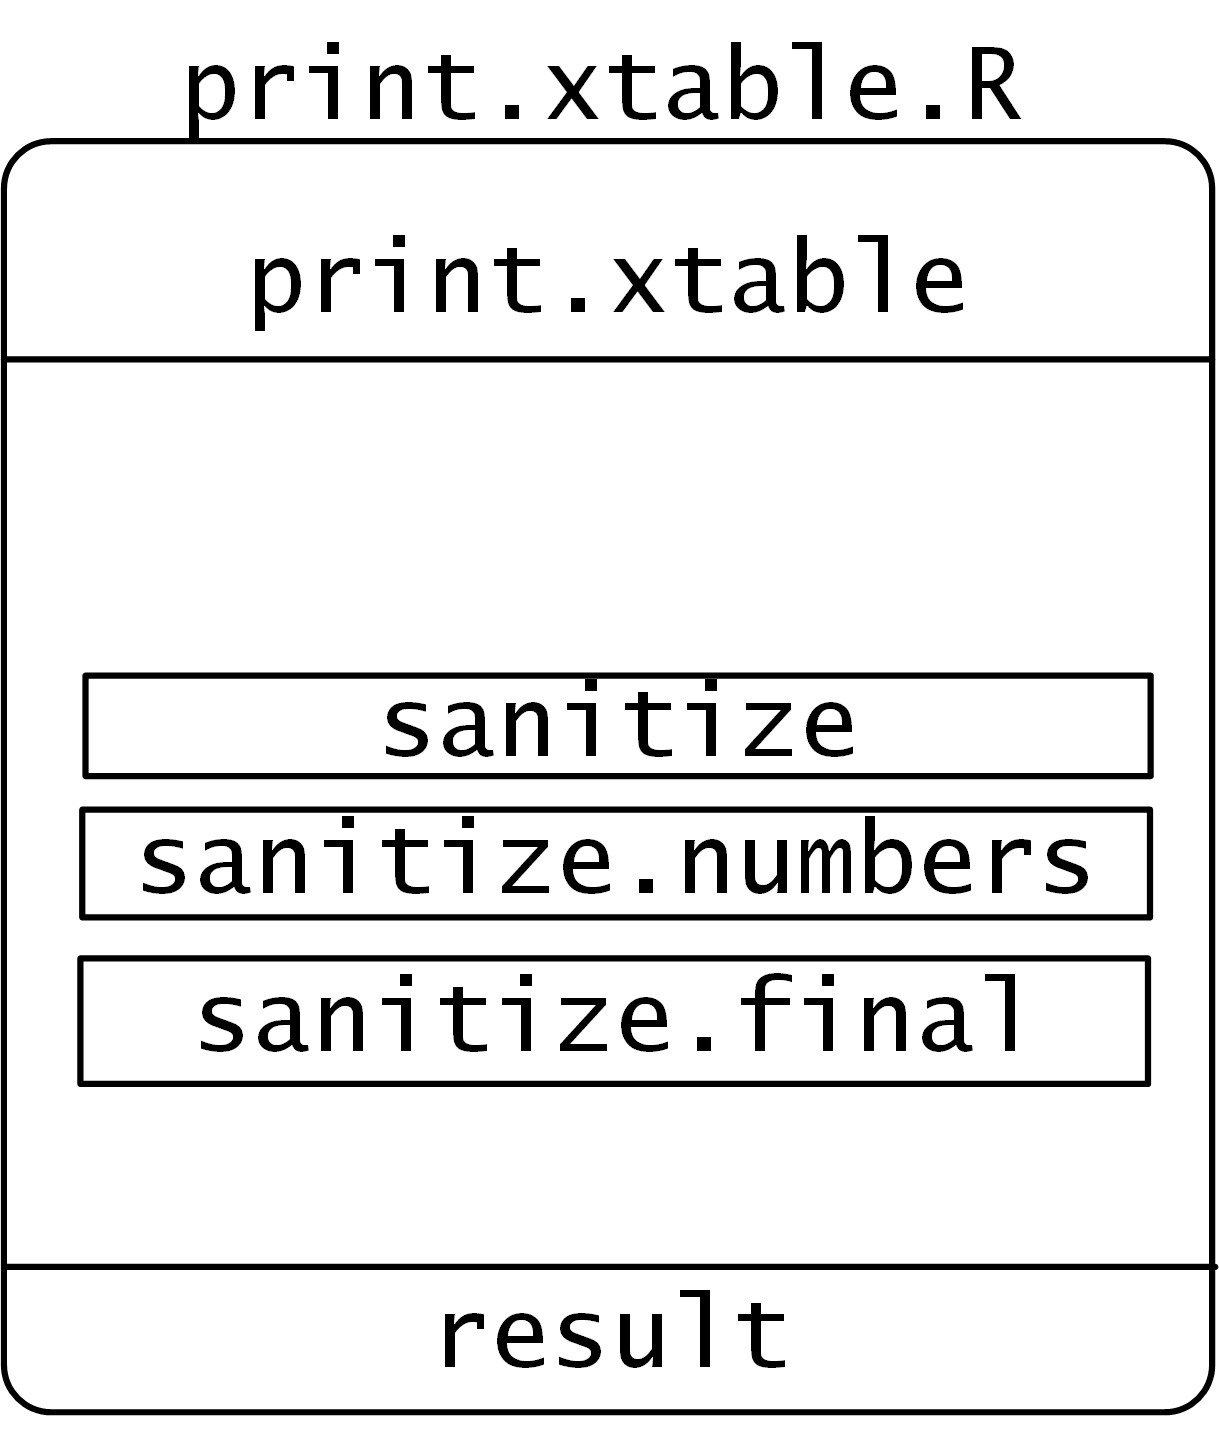
\includegraphics[width=\maxwidth]{figure/original} 

\end{knitrout}
\vspace{-110pt}
\caption{representation of \code{print.xtable} before refactoring}\label{fig:original}
\end{figure}


Having established a testing procedure, the next task was to abstract away the majority of the programmatic operations or detail within \code{print.xtable}. Separating these parts into external functions revealed more of the function's general process. It also showed that there were some lines of code located in unsuitable sections of the function. The principal example of this was the various data or input validation operations scattered throughout \code{print.xtable}. With our desire to arrange the function in a modular fashion, the validation operations were moved from their disparate areas to new validation functions. By grouping the validation operations and placing them at the start of \code{print.xtable} error messages will be returned promptly. This grouping also provides the benefit enabling us to avoid repetition of such checks because we will be able to view all of the validations at once.\\


%put in a ref to section on practice
Creating new functions was an opportunity to apply 'proper programming practice' in the naming schema. The \code{print.xtable} function has a lot of detail that is time consuming and somewhat challenging to understand. By extracting this detail to internal functions and applying appropriate names the overall activities of the \code{print.xtable} were less obscured by these details. Rather than delve into the mechanisms of a chunk of code a reader can see that a certain variable is created via a function with a descriptive name and a set of argument variables. For instance, continuing the validation example, the function \code{addToRowValidate} takes the \code{add.to.row} user argument and checks it for validity. We can deduce that the function is validating the \code{add.to.row} variable without having to look at the 20 or so lines contained within the function. The reader does not need to go through the specifics of the internal functions to understand the main function.\\ 


One issue resulting from the separation process was the necessity to rebind values of variables modified inside new functions. With the operations to variables now occurring outside of \code{print.xtable's} environment, the variables have to be returned by each internal function and have their values reassigned to the variables in the main body. This is more of an issue in the first half of the function because it involves modifying the user input variables, or creating new variables, for later use. This was not a large issue to rectify at this stage but it did add lines to the refactored main function.\\

Listing \ref{lst:addvalidate} is the \code{addToRowValidate} function that produces the errors when the \code{add.to.row} user argument is specified incorrectly. This is the function that throws the errors that are detected by the \pkg{testthat} tests in listing \ref{lst:addtorowtest}. 

\vspace{4mm}

\begin{minipage}{\linewidth}
\begin{lstlisting}[caption={add to row validation},label={lst:addvalidate},language=R]
addToRowValidate <- function(add.to.row, pos, x){
  if (is.list(add.to.row) && length(add.to.row) == 2) {
        if (is.null(names(add.to.row))) {
            names(add.to.row) <- c('pos', 'command')
        } else if (any(sort(names(add.to.row))!= c('command', 'pos'))) {
            stop("the names of the elements of 'add.to.row' must be 'pos' and 'command'")
        }
        if (is.list(add.to.row$pos) && is.vector(add.to.row$command, mode = 'character')) {
            npos <- length(add.to.row$pos)
            if (npos != length(add.to.row$command)) {
                    stop("the length of 'add.to.row$pos' must be equal to the length of 'add.to.row$command'")
            }
            if (any(unlist(add.to.row$pos) < -1) | any(unlist(add.to.row$pos) > nrow(x))) {
                    stop("the values in add.to.row$pos must be inside the interval [-1, nrow(x)]") 
            }
        } else {
                stop("the first argument ('pos') of 'add.to.row' must be a list, the second argument ('command') must be a vector of mode character")
        }
    } else {
        stop("'add.to.row' argument must be a list of length 2")
    }
  return(list(add.to.row = add.to.row, npos =  npos))
}
\end{lstlisting}
\end{minipage}


\subsection{Diagram of first stage of refactoring}

The result of moving many of the more detailed components of the main function to separate internal functions is rendered in figure \ref{fig:firstRefactor}. The number of functions created demonstrates \code{print.xtable}'s excessive size and activity. Moving sections of \code{print.xtable} to an internal function file follows on from the principles outlined in section \ref{sec:practice}, on proper programming practice. The function is more compact, down to approximately 250 lines from 650, however, as in figure \ref{fig:firstRefactor}, the structure of \code{print.xtable} and its associated functions is simple and does not present a clear process. Further reorganisation from this stage is required to reduce the size of \code{print.xtable} and provide an understandable structure.

%will have to manually add float, caption and vspace
%stage1.png
\begin{figure}[H]
\vspace{-80pt}
\begin{knitrout}
\definecolor{shadecolor}{rgb}{0.969, 0.969, 0.969}\color{fgcolor}
\includegraphics[width=\maxwidth]{figure/firstRefactor} 

\end{knitrout}
\vspace{-70pt}
\caption{representation of \code{print.xtable} with programmatic detail removed to internal functions}\label{fig:firstRefactor}
\end{figure}


\section{More abstraction}

%section introduction
At this stage of refactoring, \code{print.xtable} is a sequence of function calls and subsequent assignments of variables returned from these function calls. Further refactoring required considering what each section of the code was doing and forming coherent groups. Since the \code{print.xtable} and the internal functions make up two layers, more abstraction would require a third, intermediary layer between \code{print.xtable} and the internal functions. To continue refactoring, the function can be divided into three sections. The first part is pre-processing, where the user input arguments are checked for validity and the more complex user arguments are assigned. The second contains the large \code{if else} statement that creates a large set of variables used for building the final table. In figure \ref{fig:pseudo} this consists of the central \latex and HTML 'components' sections, which total approximately 250 lines. The third and final part uses the variables created in part two, along with the pre-processed user arguments, to construct the final table. Figure \ref{fig:process} represents the three distinct sections and their relationship.\\

%put in small flow chart diagram to show rough process
%processEDIT
\begin{figure}[H]
\vspace{-110pt}
\begin{knitrout}
\definecolor{shadecolor}{rgb}{0.969, 0.969, 0.969}\color{fgcolor}
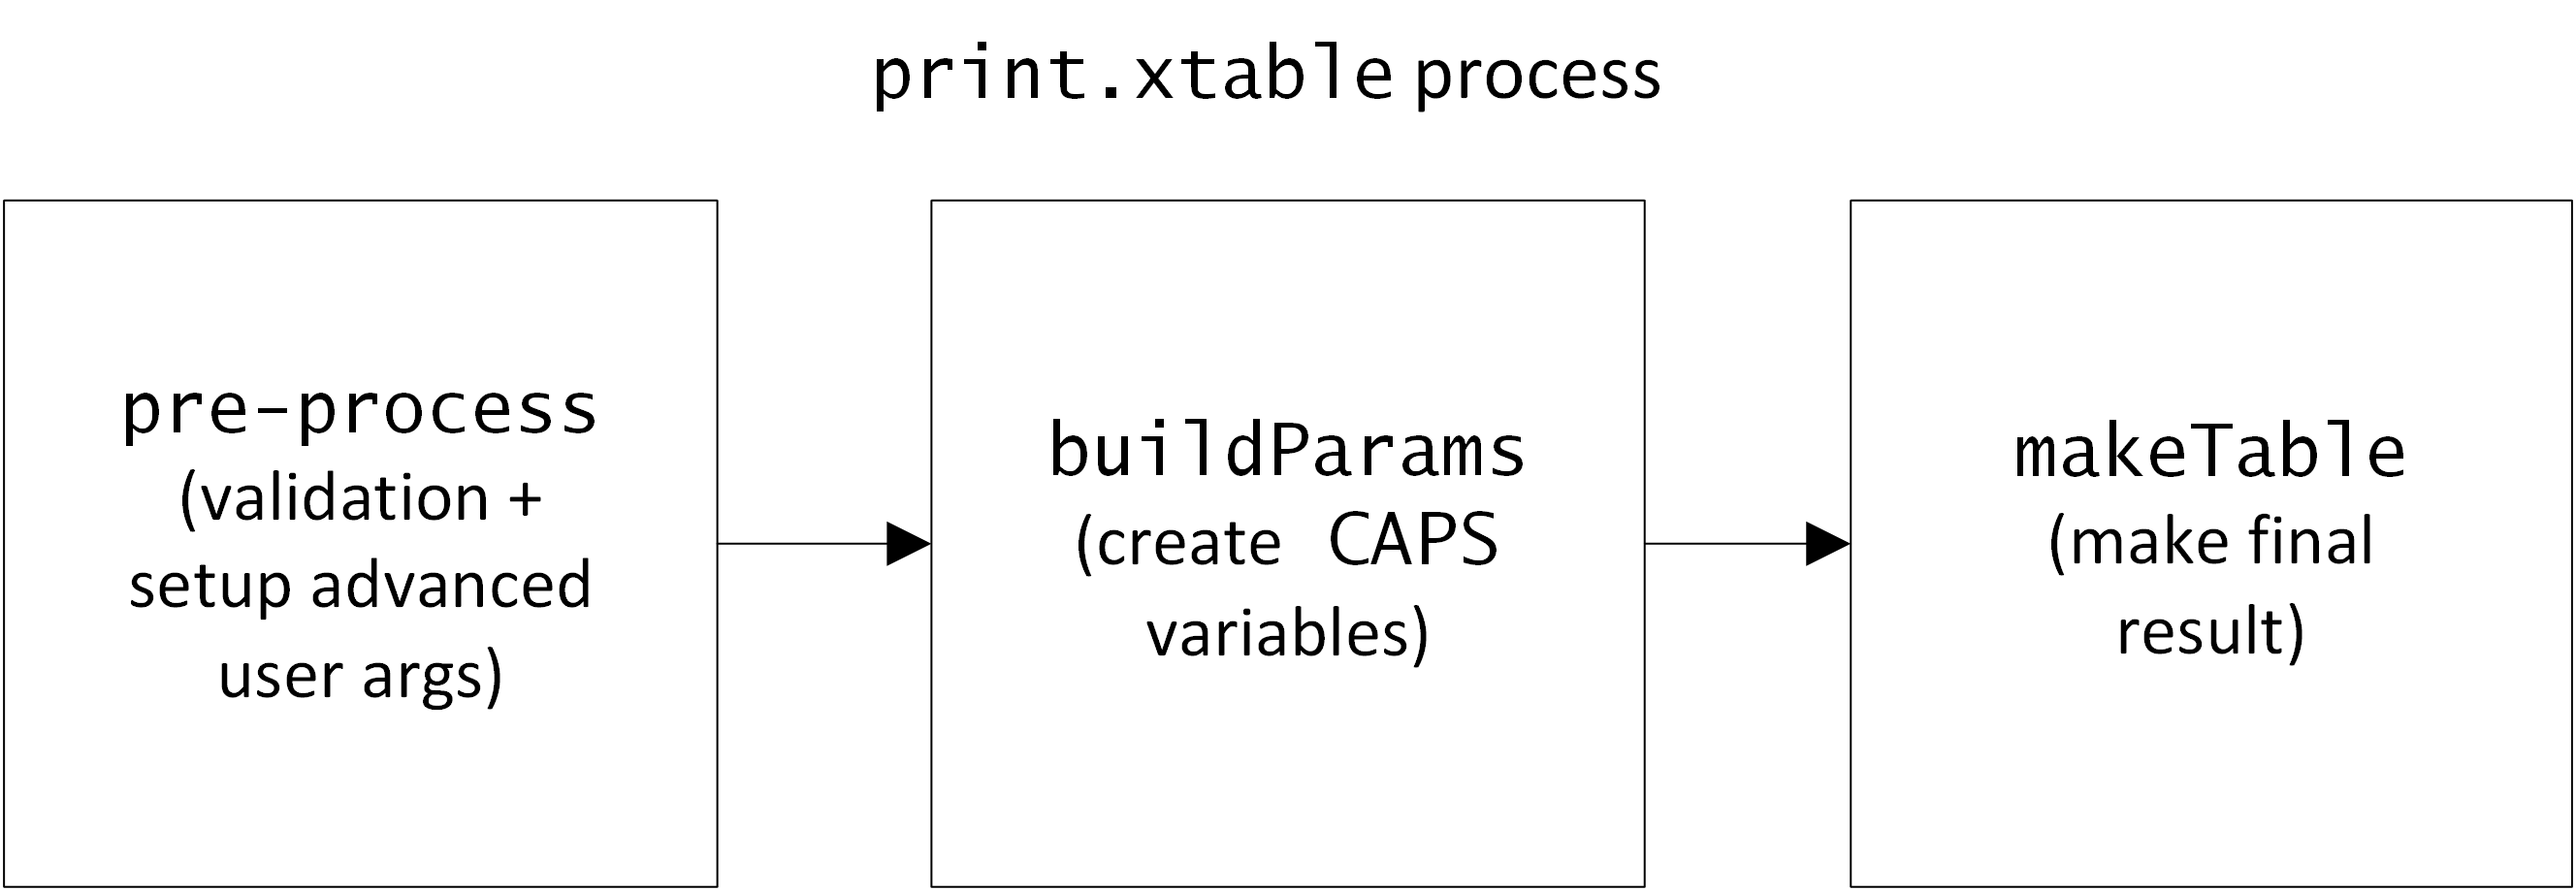
\includegraphics[width=\maxwidth]{figure/process} 

\end{knitrout}
\vspace{-100pt}
\caption{process of the \code{print.xtable} function}\label{fig:process}
\end{figure}

%part on pre-processing section - note very good
The first of these is the pre-processing section. This is the shortest and perhaps least cohesive part identified for abstraction. It contains validation functions and assignment of arguments such as \code{add.to.row} and \code{hline}. The abstraction possible here is limited by wanting to avoid excessive argument lists and reassignment of variables. The issue of variables being created or changed in this first part and then reused later in the function is the primary reason for not abstracting this section. Excluding comments and white space, this section is only 28 lines long; and therefore not as important to abstract further. It is still useful to identify this section separately from the other two sections because this enables us to partition the function into distinct sections. The drawback of this approach is leaving the pre-processing section at a different level of abstraction to the other two sections.\\

%part on buildParams section
The next section to consider from figure \ref{fig:process} is the 'buildParams' section, which consists entirely of a large \code{if else} section that generates variables used for constructing or 'building' the final table. These variables, which are created in the 'buildParams' section, number at over 20. Examples of these variables are: \code{EROW}, \code{BROW}, \code{BCAPTION} and \code{ECAPTION}, hence the label of 'CAPS' in figure \ref{fig:process}. The same set of variables are generated by the function for both \latex and HTML, with the values of the variables dependent on the type of table being produced.  Some of these variables are assigned empty values depending on whether the table type is HTML or \latex. Due to having the same variable set the HTML and \latex variable versions are used identically later in \code{print.xtable}. This identical use allowed for separate functions for \latex and HTML, so that the \code{if "latex" else "html")} structure is split. Abstracting these parts removed a large number of lines from \code{print.xtable}. As seen in the pseudo-code representation in figure \ref{fig:pseudo}, the creation of these components is a large proportion of the \code{print.xtable} function.\\

A major issue with this implementation, and with the \code{print.xtable} function in general, is the large number of parameters being returned and used in later in the function. The creation of the \code{buildParams} variables adds just over 20 variables that need to be introduced at least to the \code{print.xtable} environment. To avoid unpacking and reassigning the list of variables the \code{with} function is used in the third, \code{makeTable}, section. The advantage of using \code{with} is to be able to pass the \code{buildParams} variables into the function as a list, without extracting or manually assigning the variables within the list. This saves space in both the main and abstracted functions.\\

%can also say that with() usage possible here because we get the final result at the end of this section
The third section of \code{print.xtable} is a function utilising the \code{with} function, called 'makeTable'. This final section, which uses the extensive number of variables from 'buildParams' and the \code{print.xtable} user arguments, is a function that creates the final result. The reason we can use the \code{with} function here and not earlier in \code{print.xtable} is that we only require the \code{result} variable at the end of this new function, which is the final table to be returned. So we are not concerned with reassigning any other variables from inside the environment created by \code{with}. This final section is where the table is cobbled together from all of the components that \code{print.xtable} has been constructing. This section is identifiable because at the start an empty result variable is created, which is then built upon using the contents, columns, rows and various 'buildParams' variables until complete. This process works similarly HTML and \latex, with \latex having a few more additions. This generalised method of constructing the table, rather than having completely separate functions, is the reason for the large set of 'buildParams' variables having certain empty variables depending on the type of the table.\\

The final reorganisation step was to rearrange the internal functions into groups corresponding to the new functions. For instance, the \code{contentFormat} function was moved to the \code{makeTableInternal.R} file with the other \code{makeTable} internal functions. By grouping the internal functions by file one can go from an internal function call to the called function's body without going through a huge list of internal functions. The pre-processing section is slightly different, in that there was not an additional abstraction layer created, so the internal functions have been divided into the files \code{validation.R} and \code{preprocessInternal.R}. One interesting aspect of the \code{buildParams} internal functions, is that the HTML component has no internal functions whilst the \latex version has eight. This indicates that the HTML component for this package is somewhat lacking in user arguments.


\subsection{Diagram of refactored \code{print.xtable}}

While splitting up the refactored \code{print.xtable} into sections the internal functions were also split up into their corresponding groups. Figure \ref{fig:final} is the final refactored structure. It shows the three sections of pre-processing, buildParams and makeTable and their internal functions. Note the file names have been supplied to further illustrate how the function was divided. 
%refactored
\begin{figure}[H]
%\vspace{-30pt}
\begin{knitrout}
\definecolor{shadecolor}{rgb}{0.969, 0.969, 0.969}\color{fgcolor}
\includegraphics[width=\maxwidth]{figure/final} 

\end{knitrout}
%\vspace{-10pt}
\caption{representation of refactored \code{print.xtable}}\label{fig:final}
\end{figure}

\newpage
\section{Discussion of results}

Positives of this refactored function are:
\begin{itemize}
  \item In some sections of the function new features can easily be added.
  \item For example, if you want to expand the validation section to include checks for HTML output, you could add an HTML validation function to the \code{validation.R} file, then add the function call to \code{print.xtable}. This new validation function could then be tested by adding to the test file.
  \item \code{print.xtable} has been considerably reduced from about 650 lines to just under 110, including the original 30 plus  lines of the main function arguments and 25 lines of comments and white space.
  \item Readers can see the high level functions names and comments rather than having to unravel low level details.
\end{itemize}


\noindent Limitations of this refactoring are:
\begin{itemize}
  \item The pre-processing section is at a different level of abstraction to the other sections. Creating a function with this section would further reduce the size of \code{print.xtable}.
  \item It is difficult to elegantly or cleanly to achieve this abstraction because there would be a considerable number of variables that have to be entered as arguments into the function and then reassigned at the end of the function call.
  \item Having large blocks of arguments passed to functions is difficult to decipher. This issue is tough to avoid because \pkg{xtable} has a large number of arguments.
\end{itemize}


%include pages in reference?

\chapter{Conclusion}

This report has shown the process undertaken to modify \pkg{xtable} and refactor the function, \pkg{print.xtable}. This was done by analysing what the code does and then separating it out into functions. Once the functions were separated from the main body it was possible to further restructure the code. These rearrangements allowed the function to be structured in a more layered and organised manner. Doing this has increased our understanding of the package and how certain features can be implemented.\\ 

As evidenced from rearranging \code{print.xtable}, the lack of HTML work indicates that the HTML features are lacking. Furthermore, whilst the refactor of the code garners greater understanding, the package would ideally be rewritten from scratch. This would help alleviate issues such as the clash between certain \latex table environments while allowing for a fully fledged HTML component.\\


\backmatter

\nocite{*}
\printbibliography[title={References}]



\appendix

%\addtocontents{toc}{\setlength\cftchapternumwidth{1em}}
\renewcommand\thechapter{}
\chapter{Refactored functions}



\begin{lstlisting}
## -- print.xtable.R -- ##

print.xtable <- function(x,
  type = getOption("xtable.type", "latex"),
  file = getOption("xtable.file", ""),
  append = getOption("xtable.append", FALSE),
  floating = getOption("xtable.floating", TRUE),
  floating.environment = getOption("xtable.floating.environment", 
                                "table"),
  table.placement = getOption("xtable.table.placement", "ht"),
  caption.placement = getOption("xtable.caption.placement", 
                                "bottom"),
  caption.width = getOption("xtable.caption.width", NULL),
  latex.environments = getOption("xtable.latex.environments", 
                                 c("center")),
  tabular.environment = getOption("xtable.tabular.environment", 
                                  "tabular"),
  size = getOption("xtable.size", NULL),
  hline.after = getOption("xtable.hline.after", c(-1,0,nrow(x))),
  NA.string = getOption("xtable.NA.string", ""),
  include.rownames = getOption("xtable.include.rownames", TRUE),
  include.colnames = getOption("xtable.include.colnames", TRUE),
  only.contents = getOption("xtable.only.contents", FALSE),
  add.to.row = getOption("xtable.add.to.row", NULL),
  sanitize.text.function = 
          getOption("xtable.sanitize.text.function", NULL),
  sanitize.rownames.function = 
          getOption("xtable.sanitize.rownames.function",
          sanitize.text.function),
  sanitize.colnames.function = 
          getOption("xtable.sanitize.colnames.function",
          sanitize.text.function),
  math.style.negative = getOption("xtable.math.style.negative", 
                        FALSE),
  html.table.attributes = 
          getOption("xtable.html.table.attributes", "border=1"),
  print.results = getOption("xtable.print.results", TRUE),
  format.args = getOption("xtable.format.args", NULL),
  rotate.rownames = getOption("xtable.rotate.rownames", FALSE),
  rotate.colnames = getOption("xtable.rotate.colnames", FALSE),
  booktabs = getOption("xtable.booktabs", FALSE),
  scalebox = getOption("xtable.scalebox", NULL),
  width = getOption("xtable.width", NULL),
  comment = getOption("xtable.comment", TRUE),
  timestamp = getOption("xtable.timestamp", date()),
  ...)
{
    type <- tolower(type)

    ## validate that output type and 
    ## various latex environments are valid
    validatedVars <- envirValidate(type, floating.environment, 
                                    table.placement, 
                                    caption.placement, 
                                    tabular.environment, 
                                    floating, 
                                    hline.after, x)
    floating <- validatedVars$floating
    table.placement <- validatedVars$table.placement

    ## assign caption and short.caption from attributes for usage
    captions <- captionOrganise(x)
    short.caption <- captions$short.caption
    caption <- captions$caption

    ## Claudio Agostinelli <claudio@unive.it> 
    ## dated 2006-07-28 include.rownames,
    ## include.colnames
    pos <- 0
    if (include.rownames) pos <- 1

    ## add.to.row checks
    if (!is.null(add.to.row)) {
        ## validate that add.to.row commmands have 
        ## been entered correctly, 
        ## return add.to.row and npos
        res <- addToRowValidate(add.to.row, pos, x)
        add.to.row <- res$add.to.row
        npos <- res$npos
    } else {
        add.to.row <- list(pos = list(),command = character(0))
        npos <- 0
    }

    
    ## Add line rules to end of row (can include extra commmands 
    ## under the addtorow or hlines or booktabs rules)
    if (type == "latex") {
        ## this assigns the latex line rules depending on booktabs
        PHEADER <- lineRule(x, hline.after, booktabs)
    } else {
        PHEADER <- ""
    }

    lastcol <- rep(" ", nrow(x)+2)

    ## line rule locations assigned into add.to.row
    add.to.row <- hlineLocations(booktabs, add.to.row, 
                                 npos, hline.after, PHEADER) 

    ## assign position and command of addtorow commands
    if ( length(add.to.row$command) > 0 ) {
         addCmds <- assignAddCommands(add.to.row, lastcol)
         lastcol <- addCmds$lastcol
    }

    ## params are a set of CAPS variables used to make the table
    if (type == "latex") {
        params <- latexParams(type, tabular.environment, 
                      floating, floating.environment, 
                      table.placement, latex.environments,
                      x, include.rownames, width, 
                      caption.placement, short.caption, 
                      caption, lastcol, scalebox, 
                      size, caption.width)
    } else {
        params <- htmlParams(html.table.attributes, 
                             caption.placement, x, pos)
    }

    ## use formatted user arguments and buildParams 
    ## to make and return final table
    result <- makeTable(params, file, append, comment, 
                        type, timestamp,only.contents, 
                        floating, caption, caption.placement, 
                        x, include.colnames, include.rownames, 
                        sanitize.colnames.function, 
                        sanitize, rotate.colnames,pos, 
                        sanitize.rownames.function, 
                        rotate.rownames, format.args, 
                        sanitizeNumbers, math.style.negative, 
                        sanitize.text.function, NA.string, 
                        lastcol, tabular.environment, 
                        booktabs, PHEADER)

    if (print.results){
       print(result)
    }

    return(invisible(result$text))
}


makeTable <- function(params, file, append, comment, type, 
                      timestamp, only.contents, floating, 
                      caption, caption.placement, x, 
                      include.colnames, include.rownames, 
                      sanitize.colnames.function, sanitize, 
                      rotate.colnames,pos, 
                      sanitize.rownames.function, rotate.rownames, 
                      format.args, sanitizeNumbers, 
                      math.style.negative, sanitize.text.function, 
                      NA.string, lastcol, tabular.environment, 
                      booktabs, PHEADER){

            with(params, {
            result <- string("", file = file, append = append)
            info <- R.Version()
            ## modified Claudio Agostinelli 
            ## <claudio@unive.it> dated 2006-07-28
            ## to set automatically the package version
            if (comment){
                result <- addComment(result, BCOMMENT, type, 
                                     info, ECOMMENT, timestamp) 
            }
            ## start adding outside environment 
            ## tags; caption, label, etc.
            if (!only.contents) {                                                                 
                result <- captionAdd(result, BTABLE, BENVIRONMENT, 
                                    floating, caption, 
                                    caption.placement, type, 
                                    x, BCAPTION, ECAPTION, 
                                    BLABEL, ELABEL, BSIZE, 
                                    BTABULAR)               
            }
         
            ## update result with user defined (or default) column 
            ## specification for inclusion of names, etc.
            result <- colNames(include.colnames, result, BROW, 
                              BTH, include.rownames, type, x, 
                              STH, sanitize.colnames.function, 
                              sanitize,  rotate.colnames, 
                              ETH, EROW)                              
            cols <- matrix("", nrow = nrow(x), ncol = ncol(x)+pos)

            ## update result with user defined column 
            ## specification (inclusion, exclusion , etc.)
            if (include.rownames) {
                cols[, 1] <- rowNames(sanitize.rownames.function, 
                                      x, type, rotate.rownames,
                                      sanitize)   
            }

            ## contentFormat formats 
            ## digits and sanitization content
            varying.digits <- is.matrix( attr( x, "digits", 
                                            exact = TRUE ) )
            cols <- contentFormat(x, pos, format.args, 
                                  varying.digits, cols, 
                                  sanitize, sanitizeNumbers, 
                                  type, math.style.negative, 
                                  sanitize.text.function, 
                                  NA.string) 

            ## uses Params that seperate rows, values to 
            ## create matrix used for constructing final result
            full <- addSeparators(x, pos, BTD1, BTD2, BTD3, cols, 
                                  ETD, EROW, lastcol, BROW)

            if (type == "latex") full[, 2] <- ""
            result <- result + lastcol[2] + paste(t(full), collapse = "")

            ## add final environments and make adjustments 
            ## if they are longtable or floating
            if (!only.contents) {
                if (tabular.environment == "longtable") {
                    ltRes <- longtableFinal(booktabs, result, 
                                  PHEADER, caption.placement, 
                                  caption,type, BCAPTION, 
                                  ECAPTION, x, BLABEL, ELABEL)  
                    result <- ltRes$result
                    ETABULAR <- ltRes$ETABULAR
                }
                result <- result + ETABULAR
                result <- result + ESIZE
                if ( floating == TRUE ) {
                    result <- floatingFinal(caption, type, 
                                            caption.placement, 
                                            result,BCAPTION, 
                                            ECAPTION, x, 
                                            BLABEL, ELABEL)
                }
                result <- result + EENVIRONMENT
                result <- result + ETABLE
              }
              result <- sanitizeFinal(result, type)
            })
    }
\end{lstlisting}

\begin{lstlisting}

## -- preprocessInternal.R -- ##

## If caption is length 2, treat the 
## second value as the "short caption"
captionOrganise <- function(x){
  caption <- attr(x, "caption", exact = TRUE)
  short.caption <- NULL
  if (!is.null(caption) && length(caption) > 1){
    short.caption <- caption[2]
    caption <- caption[1]
  }
  return(list(caption = caption, short.caption = short.caption))
}


## assign appropriate LaTeX line rules
## output: PHEADER this contains the 
## line rules depending on if booktabs or not
## Claudio Agostinelli <claudio@unive.it> dated 2006-07-28 add.to.row
lineRule <- function(x, hline.after, booktabs){
  if(!booktabs){
    PHEADER <- "\\hline\n"
  } else {
    if (is.null(hline.after)){
      PHEADER <- ""
    } else {
      hline.after <- sort(hline.after)
      PHEADER <- rep("\\midrule\n", length(hline.after))
      if (hline.after[1] == -1) {
        PHEADER[1] <- "\\toprule\n"
      }
      if (hline.after[length(hline.after)] == nrow(x)) {
        PHEADER[length(hline.after)] <- "\\bottomrule\n"
      }
    }  
  }
  return(PHEADER)
}



## insert extra lineRule locations into add.to.row
hlineLocations <- function(booktabs, add.to.row, npos, 
                            hline.after, PHEADER){
  if (!is.null(hline.after)) {
    if (!booktabs){
      add.to.row$pos[[npos+1]] <- hline.after
    } else {
      for(i in 1:length(hline.after)) {
        add.to.row$pos[[npos+i]] <- hline.after[i]
      }
    }
    add.to.row$command <- c(add.to.row$command, PHEADER)
  }
  return(add.to.row)
}

#assign add commands into variables with order to be used
assignAddCommands <- function(add.to.row, lastcol){
  for (i in 1:length(add.to.row$command)) {
    addpos <- add.to.row$pos[[i]]
    freq <- table(addpos)
    addpos <- unique(addpos)
    for (j in 1:length(addpos)) {
      lastcol[addpos[j]+2] <- paste(lastcol[addpos[j]+2],
                                  paste(rep(add.to.row$command[i],
                                        freq[j]),
                                      sep = "", collapse = ""),
                                    sep = " ")
    }
  }
  return(list(addpos = addpos, freq = freq, lastcol = lastcol))
  #only lastcol is actually used again in print.xtable
}

\end{lstlisting}

\newpage

\begin{lstlisting}

## -- buildParams.R --

#create CAPS variables parameters
latexParams <- function(type, tabular.environment, floating, 
                        floating.environment, table.placement, 
                          latex.environments, x, 
                          include.rownames, width, 
                          caption.placement, short.caption, 
                          caption, lastcol, 
                          scalebox, size, caption.width)
{
        BCOMMENT <- "% "
        ECOMMENT <- "\n"
        ## See e-mail from "John S. Walker 
        ## <jsw9c@uic.edu>" dated 5-19-2003
        ## regarding "texfloat"

        if ( floating == TRUE ) {
            ## validate environments then create environment output
            fRes = floatingEnv(floating.environment, 
                              table.placement, latex.environments)
            BTABLE <- fRes$BTABLE
            ETABLE <- fRes$ETABLE
            BENVIRONMENT <- fRes$BENVIRONMENT
            EENVIRONMENT <- fRes$EENVIRONMENT
        } else {
            BTABLE <- ""
            ETABLE <- ""
            BENVIRONMENT <- ""
            EENVIRONMENT <- ""
        }

        ## index
        tmp.index.start <- indexStart(include.rownames, x)

        ## assign width argument and check it is valid
        WIDTH <- tbWidth(width, tabular.environment)

        ## add in tabular environment
        BTABULAR <- bTab(tabular.environment, WIDTH, tmp.index.start, x)

        ## fix 10-26-09 (robert.castelo@upf.edu) the following
        ## 'if' condition is added for top caption on longtable
        if (tabular.environment == "longtable" && 
            caption.placement == "top") {
            lcRes <- longCaptionTop(short.caption, caption, type)
            BCAPTION <- lcRes$BCAPTION; ECAPTION <- lcRes$ECAPTION   
            BTABULAR <- lcRes$BTABULAR
        }
        ## Claudio Agostinelli <claudio@unive.it> dated 2006-07-28
        ## add.to.row position -1
        BTABULAR <- paste(BTABULAR, lastcol[1], sep = "")
        ## the \hline at the end, if 
        ## present, is set in full matrix
        ETABULAR <- paste("\\end{", tabular.environment, "}\n", 
                                                  sep = "")

        ## Add scalebox - CR, 7/2/12
        sbRes <- scaleBox(scalebox, BTABULAR, ETABULAR)
        BTABULAR <- sbRes$BTABULAR
        ETABULAR <- sbRes$ETABULAR

        #size
        sizeRes <- sizeLatex(size)
        BSIZE <- sizeRes$BSIZE
        ESIZE <- sizeRes$ESIZE

        BLABEL <- "\\label{"
        ELABEL <- "}\n"

        capRes <- captionLatex(caption.width, short.caption)
        BCAPTION <- capRes$BCAPTION
        ECAPTION <- capRes$ECAPTION

        BROW <- ""
        EROW <- " \\\\ \n"
        BTH <- ""
        ETH <- ""
        STH <- " & "
        BTD1 <- " & "
        BTD2 <- ""
        BTD3 <- ""
        ETD  <- ""

        ## named list for usage in makeTable
        params = list(BCOMMENT = BCOMMENT, ECOMMENT = ECOMMENT, 
                      BTABLE = BTABLE, ETABLE = ETABLE, 
                      BENVIRONMENT= BENVIRONMENT, 
                      EENVIRONMENT = EENVIRONMENT, 
                      BTABULAR = BTABULAR, BCAPTION = BCAPTION, 
                      ECAPTION = ECAPTION, ETABULAR = ETABULAR,
                      BSIZE = BSIZE, ESIZE = ESIZE, 
                      BLABEL = BLABEL, ELABEL = ELABEL, 
                      BROW = BROW,EROW = EROW, BTH = BTH, 
                      ETH = ETH, STH = STH, BTD1 = BTD1, 
                      BTD2 = BTD2, BTD3 = BTD3, ETD = ETD)
        return(params)
} 


htmlParams <- function(html.table.attributes, 
                      caption.placement, x, pos){
        BCOMMENT <- "<!-- "
        ECOMMENT <- " -->\n"
        BTABLE <- paste("<TABLE ", 
                    html.table.attributes, 
                    ">\n", sep = "")
        ETABLE <- "</TABLE>\n"
        BENVIRONMENT <- ""
        EENVIRONMENT <- ""
        BTABULAR <- ""
        ETABULAR <- ""
        BSIZE <- ""
        ESIZE <- ""
        BLABEL <- "<A NAME="
        ELABEL <- "></A>\n"
        BCAPTION <- paste("<CAPTION ALIGN=\"", 
                      caption.placement, "\"> ", sep = "")
        ECAPTION <- " </CAPTION>\n"
        BROW <- "<TR>"
        EROW <- " </TR>\n"
        BTH <- " <TH> "
        ETH <- " </TH> "
        STH <- " </TH> <TH> "
        BTD1 <- " <TD align=\""
        align.tmp <- attr(x, "align", exact = TRUE)
        align.tmp <- align.tmp[align.tmp!="|"]
        BTD2 <- matrix(align.tmp[(2-pos):(ncol(x)+1)],
                       nrow = nrow(x), ncol = ncol(x)+pos, 
                       byrow = TRUE)
        ## Based on contribution from Jonathan Swinton <jonathan@swintons.net>
        ## in e-mail dated Wednesday, January 17, 2007
        BTD2[regexpr("^p", BTD2)>0] <- "left"
        BTD2[BTD2 == "r"] <- "right"
        BTD2[BTD2 == "l"] <- "left"
        BTD2[BTD2 == "c"] <- "center"
        BTD3 <- "\"> "
        ETD  <- " </TD>"
        ## list of all parameters created by assignments 
        ## above (except WIDTH and tmp.index.start)
        params = list(BCOMMENT = BCOMMENT, ECOMMENT = ECOMMENT, 
                      BTABLE = BTABLE, ETABLE = ETABLE, 
                      BENVIRONMENT= BENVIRONMENT, 
                      EENVIRONMENT = EENVIRONMENT, 
                      BTABULAR = BTABULAR, 
                      BCAPTION = BCAPTION, ECAPTION = ECAPTION, 
                      ETABULAR = ETABULAR, BSIZE = BSIZE, 
                      ESIZE = ESIZE, BLABEL = BLABEL, 
                      ELABEL = ELABEL, BROW = BROW,
                      EROW = EROW, BTH = BTH, ETH = ETH,
                      STH = STH, BTD1 = BTD1, BTD2 = BTD2, 
                      BTD3 = BTD3, ETD = ETD)
        return(params)
}
\end{lstlisting}


%buildParamsInternal.R
\begin{lstlisting}
## -- buildParamsInternal.R --

## buildFunctions: where CAPS variables 
## used in output are created

## floating function: assign the user supplied 
## environments into vars for use in output
floatingEnv <- function(floating.environment, table.placement, latex.environments) {
    ## See e-mail from "Pfaff, Bernhard <Bernhard.Pfaff@drkw.com>"
    ## dated 7-09-2003 regarding "suggestion for an amendment of
    ## the source"
    ## See e-mail from "Mitchell, David"
    ## <David.Mitchell@dotars.gov.au>" dated 2003-07-09 regarding
    ## "Additions to R xtable package"
    ## See e-mail from "Garbade, Sven"
    ## <Sven.Garbade@med.uni-heidelberg.de> dated 2006-05-22
    ## regarding the floating environment.
    BTABLE <- paste("\\begin{", floating.environment, "}",
                    ifelse(!is.null(table.placement),
                          paste("[", table.placement, "]", 
                          sep = ""), ""), "\n", sep = "")
    if ( is.null(latex.environments) || 
       (length(latex.environments) == 0) ) {
      BENVIRONMENT <- ""
      EENVIRONMENT <- ""
    } else {
      BENVIRONMENT <- ""
      EENVIRONMENT <- ""
      if ("center" %in% latex.environments){
        BENVIRONMENT <- paste(BENVIRONMENT, 
                            "\\centering\n", sep = "")
      }
      for (i in 1:length(latex.environments)) {
        if (latex.environments[i] == "") next
        if (latex.environments[i] != "center"){
          BENVIRONMENT <- paste(BENVIRONMENT,
                                "\\begin{", latex.environments[i],
                                "}\n", sep = "")
          EENVIRONMENT <- paste("\\end{", latex.environments[i],
                                "}\n", EENVIRONMENT, sep = "")
        }
      }
    }
    ETABLE <- paste("\\end{", floating.environment, 
                                    "}\n", sep = "")
    
    return(list(BTABLE = BTABLE, ETABLE = ETABLE, 
                BENVIRONMENT = BENVIRONMENT, 
                EENVIRONMENT = EENVIRONMENT))
}


indexStart <- function(include.rownames, x){
        tmp.index.start <- 1
        if (!include.rownames) {
            while ( attr(x, "align", 
                   exact = TRUE)[tmp.index.start] == '|' )
                tmp.index.start <- tmp.index.start + 1
            tmp.index.start <- tmp.index.start + 1
        }
        return(tmp.index.start)
}

## Added "width" argument for use with "tabular*" or
## "tabularx" environments - CR, 7/2/12t
## check that width and longtable aren't
## both used, plus assign width argument
tbWidth <- function(width, tabular.environment){
    if (is.null(width)){
      WIDTH <-""
    } else if (is.element(tabular.environment, c("tabular", "longtable"))){
        warning("Ignoring 'width' argument.  The 'tabular' and 
                'longtable' environments do not support a width 
                  specification.  Use another environment such as 
                  'tabular*' or 'tabularx' to specify the width.")
        WIDTH <- ""
    } else {
        WIDTH <- paste("{", width, "}", sep = "")
    }
    return(WIDTH)
}


## BTABULAR function
bTab <- function(tabular.environment, WIDTH, tmp.index.start, x){
    paste("\\begin{", tabular.environment, "}",
          WIDTH, "{",
          paste(c(attr(x, "align",
                       exact = TRUE)[
                       tmp.index.start:length(attr(x, "align",
                                              exact = TRUE))],
                  "}\n"),
                sep = "", collapse = ""),
          sep = "")
}



## fix 10-26-09 (robert.castelo@upf.edu) the following
## 'if' condition is added here to support
## a caption on the top of a longtable
longCaptionTop <- function(short.caption, caption, type){
        if (is.null(short.caption)){
            BCAPTION <- "\\caption{"
        } else {
            BCAPTION <- paste("\\caption[", 
                              short.caption, "]{", sep = "")
        }
        ECAPTION <- "} \\\\ \n"
        if ((!is.null(caption)) && (type == "latex")) {
            BTABULAR <- paste(BTABULAR,  BCAPTION, 
                              caption, ECAPTION,
                              sep = "")
        }
        return(list(BCAPTION = BCAPTION, ECAPTION = ECAPTION, 
                    BTABULAR = BTABULAR))
}


## scalebox
scaleBox <- function(scalebox, BTABULAR, ETABULAR){
      if (!is.null(scalebox)){
          BTABULAR <- paste("\\scalebox{", scalebox, 
                            "}{\n", BTABULAR, sep = "")
          ETABULAR <- paste(ETABULAR, "}\n", sep = "")
      }
      return(list(BTABULAR = BTABULAR, ETABULAR = ETABULAR))
}

## size
sizeLatex <- function(size){
      ## BSIZE contributed by Benno 
      ## <puetz@mpipsykl.mpg.de> in e-mail
      ## dated Wednesday, December 01, 2004
      if (is.null(size) || !is.character(size)) {
          BSIZE <- ""
          ESIZE <- ""
      } else {
          if(length(grep("^\\\\", size)) == 0){
              size <- paste("\\", size, sep = "")
          }
          BSIZE <- paste("{", size, "\n", sep = "")
          ESIZE <- "}\n"
      }
      return(list(BSIZE = BSIZE, ESIZE = ESIZE))
}


captionLatex <- function(caption.width, short.caption){
      ## Added caption width (jeff.laake@nooa.gov)
      if(!is.null(caption.width)){
          BCAPTION <- paste("\\parbox{",caption.width,"}{",sep="")
          ECAPTION <- "}"
      } else {
          BCAPTION <- NULL
          ECAPTION <- NULL
      }
      if (is.null(short.caption)){
       BCAPTION <- paste(BCAPTION,"\\caption{",sep="")
      } else {
       BCAPTION <- paste(BCAPTION,"\\caption[", short.caption, "]{", sep="")
      }
      ECAPTION <- paste(ECAPTION,"} \n",sep="")
      return(list(BCAPTION=BCAPTION, ECAPTION=ECAPTION))
}
\end{lstlisting}


%sanitize.R
\begin{lstlisting}
## -- sanitize.R --

## Based on contribution from Jonathan Swinton
## <jonathan@swintons.net> in e-mail 
## dated Wednesday, January 17, 2007

sanitize <- function(str, type) {
    if(type == "latex"){
        result <- str
        result <- gsub("\\\\", "SANITIZE.BACKSLASH", result)
        result <- gsub("$", "\\$", result, fixed = TRUE)
        result <- gsub(">", "$>$", result, fixed = TRUE)
        result <- gsub("<", "$<$", result, fixed = TRUE)
        result <- gsub("|", "$|$", result, fixed = TRUE)
        result <- gsub("{", "\\{", result, fixed = TRUE)
        result <- gsub("}", "\\}", result, fixed = TRUE)
        result <- gsub("%", "\\%", result, fixed = TRUE)
        result <- gsub("&", "\\&", result, fixed = TRUE)
        result <- gsub("_", "\\_", result, fixed = TRUE)
        result <- gsub("#", "\\#", result, fixed = TRUE)
        result <- gsub("^", "\\verb|^|", result, fixed = TRUE)
        result <- gsub("~", "\\~{}", result, fixed = TRUE)
        result <- gsub("SANITIZE.BACKSLASH", "$\\backslash$", 
                      result, fixed = TRUE)
        return(result)
    } else {
        result <- str
        ## Changed as suggested in bug report #2795
        ## That is replacement of "&" is "&amp;"
        ## instead of previous "&amp" etc
        ## result <- gsub("&", "&amp ", result, fixed = TRUE)
        ## result <- gsub(">", "&gt ", result, fixed = TRUE)
        ## result <- gsub("<", "&lt ", result, fixed = TRUE)
        result <- gsub("&", "&amp;", result, fixed = TRUE)
        result <- gsub(">", "&gt;", result, fixed = TRUE)
        result <- gsub("<", "&lt;", result, fixed = TRUE)
        ## Kurt Hornik <Kurt.Hornik@wu-wien.ac.at> on 2006/10/05
        ## recommended not escaping underscores.
        ## result <- gsub("_", "\\_", result, fixed=TRUE)
        return(result)
    }
}


sanitizeNumbers <- function(x, type, math.style.negative){
    if (type == "latex"){
        result <- x
        if ( math.style.negative ) {
        ## Jake Bowers <jwbowers@illinois.edu> in e-mail
        ## from 2008-08-20 suggested disabling 
        ## this feature to avoid
        ## problems with LaTeX's dcolumn package.
        ## by Florian Wickelmaier 
        ## <florian.wickelmaier@uni-tuebingen.de>
        ## in e-mail from 2008-10-03 requested the 
        ## ability to use the
        ## old behavior.
            for(i in 1:length(x)) {
                result[i] <- gsub("-", "$-$", result[i], 
                  fixed = TRUE)
            }
        }
    return(result)
    } else {
        return(x)
    }
}


sanitizeFinal <- function(result, type){
    if (type == "latex"){
        return(result)
    } else {
        ## Suggested by Uwe Ligges 
        ## <ligges@statistik.uni-dortmund.de>
        ## in e-mail dated 2005-07-30.
        result$text <- gsub("  *", " ",  result$text, 
                            fixed = TRUE)
        result$text <- gsub(' align="left"',  "", 
                            result$text, fixed = TRUE)
        return(result)
    }
}
\end{lstlisting}

%makeTableInternal
\begin{lstlisting}
## -- makeTableInternal --

## final part of print.xtable; 
## uses preprocessed user args and CAPS 
## variables from buildFunctions

## include R-version, package version, timestamp 
## at top of table in commented form
addComment <- function(result, BCOMMENT, type, info, 
                      ECOMMENT, timestamp){
    result <- result + BCOMMENT + type + " table generated in " +
        info$language + " " + info$major + "." + info$minor +
        " by xtable " +  packageDescription('xtable')$Version +
        " package" + ECOMMENT
    if (!is.null(timestamp)){
        result <- result + BCOMMENT + timestamp + ECOMMENT    
    }
}


## Claudio Agostinelli <claudio@unive.it> 
## dated 2006-07-28 only.contents
captionAdd <- function(result, BTABLE, BENVIRONMENT, floating, 
                      caption, caption.placement, type, 
                      x, BCAPTION, ECAPTION, BLABEL, ELABEL, 
                      BSIZE, BTABULAR) {
    result <- result + BTABLE
    result <- result + BENVIRONMENT
    if ( floating == TRUE ) {
        if ((!is.null(caption)) &&
            (type == "html" ||caption.placement == "top")) {
            result <- result + BCAPTION + caption + ECAPTION
        }
        if (!is.null(attr(x, "label", exact = TRUE)) &&
            (type == "latex" && caption.placement == "top")) {
            result <- result + BLABEL +
                      attr(x, "label", exact = TRUE) + ELABEL
        }
    }
    result <- result + BSIZE
    result <- result + BTABULAR
    return(result)
}

## Claudio Agostinelli <claudio@unive.it> dated 2006-07-28
## create and sanitize column names (CNAMES)
colNames <- function(include.colnames, result, BROW, BTH, 
                     include.rownames, type, x,
                      STH, sanitize.colnames.function, 
                      sanitize, rotate.colnames, ETH, EROW){
        if (include.colnames) {
            result <- result + BROW + BTH
            if (include.rownames) {
                 result <- result + STH
            }
            ## David G. Whiting in e-mail 2007-10-09
            if (is.null(sanitize.colnames.function)) {
                 CNAMES <- sanitize(names(x), type)
            } else {
                 CNAMES <- sanitize.colnames.function(names(x))
            }
            if (rotate.colnames) {
                 ##added by Markus Loecher, 2009-11-16
                CNAMES <- paste("\\begin{sideways}", 
                                CNAMES, "\\end{sideways}")
            }
            result <- result + paste(CNAMES, collapse = STH)
            result <- result + ETH + EROW
        } else {
            CNAMES <- NULL
            result <- result + paste(CNAMES, collapse = STH)
            result <- result + ETH 
        }
        return(result)
 }



## create and sanitize rownames (RNAMES)
rowNames <- function(sanitize.rownames.function, x, type, rotate.rownames,sanitize){
    ## David G. Whiting in e-mail 2007-10-09
    if (is.null(sanitize.rownames.function)) {
        RNAMES <- sanitize(row.names(x), type)
    } else {
        RNAMES <- sanitize.rownames.function(row.names(x))
    }
    if (rotate.rownames) {
        ##added by Markus Loecher, 2009-11-16
        RNAMES <- paste("\\begin{sideways}", 
                        RNAMES, "\\end{sideways}")
    }
    return(RNAMES)
}



## Code for letting "digits" be a matrix was provided by
## Arne Henningsen <ahenningsen@agric-econ.uni-kiel.de>
## in e-mail dated 2005-06-04.
## if( !varying.digits ) {
## modified Claudio Agostinelli 
## <claudio@unive.it> dated 2006-07-28
##  attr(x,"digits") <- matrix( attr( x, "digits",exact=TRUE ),
## nrow = nrow(x), ncol = ncol(x)+1, byrow = TRUE )

contentFormat = function(x, pos, format.args, varying.digits, 
                        cols,sanitize, sanitizeNumbers, 
                        type, math.style.negative,
                        sanitize.text.function, NA.string) {
    for(i in 1:ncol(x)) {   
        xcol <- x[, i]
        if(is.factor(xcol))
            xcol <- as.character(xcol)
        if(is.list(xcol)) {
            xcol <- sapply(xcol, unlist)
        }
        ina <- is.na(xcol)
        is.numeric.column <- is.numeric(xcol)
        if(is.character(xcol)) {
            cols[, i+pos] <- xcol
        } else {
            if (is.null(format.args)){
                format.args <- list()
            }
            if (is.null(format.args$decimal.mark)){
                format.args$decimal.mark <- options()$OutDec
            }
            if(!varying.digits){
                curFormatArgs <-  c(list(x = xcol,
                    format =
                     ifelse(attr(x, "digits", 
                            exact = TRUE )[i+1] < 0, "E",
                            attr(x, "display", exact = TRUE )[i+1]),
                        digits = abs(attr(x, "digits", 
                                  exact = TRUE )[i+1])),
                        format.args)
                cols[, i+pos] <- do.call("formatC", curFormatArgs)
            }else{
                for( j in 1:nrow( cols ) ) {
                    curFormatArgs <- c(list(x = xcol[j],
                        format =  ifelse(attr(x, "digits", 
                                  exact = TRUE )[j, i+1] < 0,
                                  "E", attr(x, "display", 
                                  exact = TRUE )[i+1]),
                                  digits = abs(attr(x, "digits", 
                                  exact = TRUE )[j, i+1])),
                                  format.args)
               cols[j, i+pos] <- do.call("formatC", curFormatArgs)
                  }
            }
      }
      ## End Ian Fellows changes
      if ( any(ina) ) cols[ina, i+pos] <- NA.string
      ## Based on contribution from Jonathan Swinton <jonathan@swintons.net>
      ## in e-mail dated Wednesday, January 17, 2007
      if ( is.numeric.column ) {
          cols[, i+pos] <- sanitizeNumbers(cols[, i+pos], 
                                      type, math.style.negative)
      } else {
          if (is.null(sanitize.text.function)) {
             cols[, i+pos] <- sanitize(cols[, i+pos], type)
          } else {
             cols[, i+pos] <- 
                      sanitize.text.function(cols[, i+pos])
          }
      }
    }
    return(cols)
}

## build up matrix with the params variables 
## for use with result variable
addSeparators <- function(x, pos, BTD1, BTD2, BTD3, cols, 
                          ETD, EROW, lastcol, BROW){
    multiplier <- 5
    full <- matrix("", nrow = nrow(x), 
                   ncol = multiplier*(ncol(x)+pos)+2)
    full[, 1] <- BROW
    full[, multiplier*(0:(ncol(x)+pos-1))+2] <- BTD1
    full[, multiplier*(0:(ncol(x)+pos-1))+3] <- BTD2
    full[, multiplier*(0:(ncol(x)+pos-1))+4] <- BTD3
    full[, multiplier*(0:(ncol(x)+pos-1))+5] <- cols
    full[, multiplier*(0:(ncol(x)+pos-1))+6] <- ETD

    full[, multiplier*(ncol(x)+pos)+2] <- 
                    paste(EROW, lastcol[-(1:2)], sep = " ")
    return(full)

}


longtableFinal <- function(booktabs, result, PHEADER, 
                           caption.placement, caption,
                           type, BCAPTION, ECAPTION, x, 
                           BLABEL, ELABEL, tabular.environment){
              ## booktabs change added the if() - 1 Feb 2012
              if(!booktabs) {
                  result <- result + PHEADER
              }

              ## fix 10-27-09 Liviu Andronic 
              ## (landronimirc@gmail.com) the
              ## following 'if' condition is inserted 
              ## in order to avoid that bottom caption 
              ## interferes with a top caption of a longtable
              if(caption.placement == "bottom"){
                  if ((!is.null(caption)) && (type == "latex")) {
                      result <- result + BCAPTION + 
                                caption + ECAPTION
                  }
              }
              if (!is.null(attr(x, "label", exact = TRUE))) {
                  result <- result + BLABEL + 
                            attr(x, "label", exact = TRUE) + ELABEL
              }
              ETABULAR <- "\\end{longtable}\n"
              return(list(result = result, ETABULAR = ETABULAR))   
}


floatingFinal <- function(caption, type, caption.placement,result,
                          BCAPTION, ECAPTION, x, BLABEL, ELABEL){
            if ((!is.null(caption)) &&
                   (type == "latex" && 
                    caption.placement == "bottom")) {
              result <- result + BCAPTION + caption + ECAPTION
            }
            if (!is.null(attr(x, "label", exact = TRUE)) &&
                caption.placement == "bottom") {
                result <- result + BLABEL + 
                          attr(x, "label", exact = TRUE) +
                          ELABEL
            }
            return(result)
}
\end{lstlisting}

\renewcommand\thechapter{}
\chapter{Test code}

\begin{lstlisting}
## -- testthat tests --

#captions
context("caption errors")
test_that("test caption errors work",{
  data(tli)
  expect_that(xtable(tli[1:10,], 
              caption = c("One", "Two", "Three")), 
              throws_error())
})


context("add to Row validation")
test_that("Check add to row fails",{
  data(tli)
  tli.table <- xtable(tli[1:10,])
  #pos not a list
  expect_that(print(tli.table, 
              add.to.row = list(pos=10, 
                command = c("&", "%^"))),
              throws_error())
  #command not a vector
  expect_that(print(tli.table, 
              add.to.row = list(pos = list(10), 
                command = list(" & "))),
              throws_error())
  #names of list elements wrong
  expect_that(print(tli.table, 
              add.to.row = list(position = list(10), 
                com = c(" & "))),
              throws_error())
  #pos and command different lengths
  expect_that(print(tli.table, 
              add.to.row = list(pos = list(5, 7, 8), 
                command = c(" & "))),
              throws_error())
  #pos numbers are higher than there are rows in data
  expect_that(print(tli.table, 
              add.to.row= list(pos = list(14,15,16), 
                command = c("%","#","^"))),
              throws_error())
  #pos negative
  expect_that(print(tli.table, 
              add.to.row = list(pos = list(-4,4), 
                command = c(" % ", "&"))),
              throws_error())
  #add.to.row argument not a list of length 2
  expect_that(print(tli.table, 
              add.to.row = list(pos = list(3), 
                command = c("&"), hline="s")),
              throws_error())
})



## test functions: addToRowValidate, 
## hlineLocations, assignAddCommands
## from this example
## http://stackoverflow.com/questions/19846796/adding-titles-to-xtable
## by Christopher Louden
test_that("Check add to row works", {
  Grade3 <- c("A","B","B","A","B","C","C","D","A",
          "B","C","C","C","D","B","B","D","C","C","D")
  Grade6 <- c("A","A","A","B","B","B","B","B","C","C",
            "A","C","C","C","D","D","D","D","D","D")
  Cohort <- table(Grade3,Grade6)
  addtorow <- list()
  addtorow$pos <- list()
  addtorow$pos[[1]] <- 0
  addtorow$pos[[2]] <- 0
  addtorow$command <- c('& \\multicolumn{4}{c}{Grade 6} \\\\\n', 
                       "Grade 3 & A & B & C & D \\\\\n")
  expect_true({capture.output(print(xtable(Cohort, 
                    caption = 'My Title'), 
                    caption.placement = 'top', 
                    add.to.row = addtorow, 
                    include.colnames = FALSE, 
                    comment = FALSE, timestamp = NULL)); TRUE})
})



context("hline after")
## test the hline after being input unsorted; tests hlineLocations
test_that("Check hline.after works and fails",{
  data(tli)
  tli.table <- xtable(tli[1:10,])
  ## check that hline order doesn't change anything
  ## this also checks that hline after works
  expect_that(capture.output(print(tli.table, 
                              hline.after = c(3,5,7))), 
              equals(capture.output(print(tli.table, 
                              hline.after = c(5, 3, 7)))))
  ## check that negative out of range (-2 or lower) throws error
  expect_that(print(tli.table, hline.after = c(-2,3,5)),
              throws_error())
  ## check that positive out of range 
  ## (greater than max rows) throws error
  expect_that(print(tli.table, hline.after = c(3,5,20)),
              throws_error())
})

context("environment validation")

## tests envirValidate is rejecting correctly
test_that("Check that the envirValidate fails invalid inputs", {
  data(tli)
  tli.table <- xtable(tli[1:10,])
  ## length of type greater than 1
  expect_that(print(tli.table, 
          type = c("latex", "html")), throws_error())
  ## type isn't anything meaningful
  expect_that(print(tli.table, type = "wrong type"), 
          throws_error())
  ## type is wrong type
  expect_that(print(tli.table, type = 1), throws_error())
  ## margintable plus tableplacement
  expect_that(print(tli.table, 
              floating.environment = "margintable", 
              table.placement = "htb"), gives_warning())
  ## table.placement wrong letters
  expect_that(print(tli.table, table.placement = "xyz"), throws_error())
  ## caption placement wrong name
  tli.table <- xtable(tli[1:10,], caption = "stuff")
  expect_that(print(tli.table, 
              caption.placement = c("side")), 
              throws_error())
})

## tbWidth
test_that("Width warning works", {
  data(tli)
  tli.table <- xtable(tli[1:10,])
  #check that width plus longtable gives warning
  expect_that(print(tli.table, tabular.environment = "longtable", width = 3, floating = FALSE),
              gives_warning())
})

## longCheck
test_that("Long table warning works", {
  data(tli)
  tli.table <- xtable(tli[1:10,])
  #check floating + longtable gives warning
  expect_that(print(tli.table, 
                tabular.environment = "longtable", 
                floating = TRUE),
              gives_warning())
})
\end{lstlisting}

\newpage

\begin{lstlisting}
## -- diff testing procedure --

## note: since using this test procedure 
##        the vignette has been updated to knitr

## create initial .tex file for testing
## Do this once, if a .tex file is not included
## with the package dist
setwd("##directory for testing new tex file")
## install current package distribution
library(xtable)
Sweave(file = "##directory/xtableGallery.snw")
file.remove("##directory/xtableGallery-concordance.tex")
file.rename("xtableGallery.tex", "xtableGalleryOriginal.tex")
detach("package:xtable", unload = TRUE)

## create a diff function to test easily
diff <- function(){
  setwd("##directory of xtableGalleryOriginal.tex")
  out <- capture.output(Sweave(file = "##dir/xtableGallery.snw"))
  out1 <- file.remove("##dir/xtableGallery-concordance.tex")
  out2 <- file.rename("xtableGallery.tex", "xtableGalleryNew.tex"
  system('##your_diff xtableGalleryNew.tex xtableGalleryOriginal.tex')
}

## can set set.seed() and options(xtable.timestamp="") 
## inside .Swn or .Rnw
\end{lstlisting}


\end{document}
